%=============================================================
%  MEMORIA TFG - SCHOOLEDULE
%  Autor: Rafael Medina Ayuso
%  Tutor: David Valbuena Segura
%  Ciclo: Desarrollo de Aplicaciones Multiplataforma (DAM)
%=============================================================

\documentclass[12pt, a4paper]{report}

%-------------------------------------------------------------
% PAQUETES
%-------------------------------------------------------------
\usepackage[utf8]{inputenc}
\usepackage[T1]{fontenc}
\usepackage[spanish]{babel}
\usepackage{geometry}
\usepackage{graphicx}
\usepackage[hyphens]{url}
\usepackage{hyperref}
\usepackage{xcolor}
\usepackage{booktabs}
\usepackage{longtable}
\usepackage{array}
\usepackage{tabularx}
\usepackage{enumitem}
\usepackage{fancyhdr}
\usepackage{titlesec}
\usepackage{parskip}
\usepackage{setspace}
\usepackage{lmodern}
\usepackage{microtype}
\usepackage{listings}
\usepackage{caption}
\usepackage{float}
\usepackage{subcaption}

% Ruta de imagenes (misma carpeta que el .tex)
\graphicspath{{./}}

%-------------------------------------------------------------
% CONFIGURACION DE PAGINA
%-------------------------------------------------------------
\geometry{
  a4paper,
  top=2.5cm,
  bottom=2.5cm,
  left=3cm,
  right=2.5cm
}

\onehalfspacing

%-------------------------------------------------------------
% COLORES
%-------------------------------------------------------------
\definecolor{azulTFG}{RGB}{0, 70, 127}
\definecolor{grisClaro}{RGB}{245, 245, 245}
\definecolor{grisTexto}{RGB}{80, 80, 80}

%-------------------------------------------------------------
% HIPERVíNCULOS
%-------------------------------------------------------------
\hypersetup{
  colorlinks=true,
  linkcolor=azulTFG,
  urlcolor=azulTFG,
  citecolor=azulTFG,
  pdftitle={Memoria TFG - Schooledule},
  pdfauthor={Rafael Medina Ayuso}
}

%-------------------------------------------------------------
% CABECERAS Y PIES
%-------------------------------------------------------------
\pagestyle{fancy}
\fancyhf{}
\fancyhead[L]{\small\textcolor{grisTexto}{Schooledule -- Memoria TFG}}
\fancyhead[R]{\small\textcolor{grisTexto}{Rafael Medina Ayuso}}
\fancyfoot[C]{\thepage}
\renewcommand{\headrulewidth}{0.4pt}

%-------------------------------------------------------------
% ESTILOS DE TITULOS
%-------------------------------------------------------------
\titleformat{\chapter}[display]
  {\normalfont\Large\bfseries\color{azulTFG}}
  {\chaptertitlename\ \thechapter}{10pt}{\huge}
\titlespacing*{\chapter}{0pt}{-20pt}{20pt}

\titleformat{\section}
  {\normalfont\large\bfseries\color{azulTFG}}
  {\thesection}{1em}{}

\titleformat{\subsection}
  {\normalfont\normalsize\bfseries}
  {\thesubsection}{1em}{}

\titlespacing*{\section}{0pt}{14pt}{6pt}
\titlespacing*{\subsection}{0pt}{10pt}{4pt}
\titlespacing*{\subsubsection}{0pt}{8pt}{3pt}

% Evitar desbordamiento de lineas con nombres largos y rutas
\setlength{\emergencystretch}{3em}
\hyphenpenalty=500
\tolerance=1500

%-------------------------------------------------------------
% CODIGO FUENTE
%-------------------------------------------------------------
\lstset{
  backgroundcolor=\color{grisClaro},
  basicstyle=\ttfamily\small,
  breaklines=true,
  frame=single,
  rulecolor=\color{gray},
  captionpos=b
}

% Logo helper para la tabla de tecnologias
\newcommand{\logo}[1]{%
  \includegraphics[height=1cm,keepaspectratio]{#1}%
}

%=============================================================
% DOCUMENTO
%=============================================================
\begin{document}

%-------------------------------------------------------------
% PORTADA
%-------------------------------------------------------------
\begin{titlepage}
  \centering
  {\Large Trabajo de Fin de Grado}\\[0.3cm]
  {\large Ciclo Formativo de Grado Superior}\\[0.3cm]
  {\large Desarrollo de Aplicaciones Multiplataforma (DAM)}\\[2cm]

  
\includegraphics[width=0.55\textwidth]{image19.png}\\[1.5cm]


  \begin{tabular}{ll}
    \textbf{Autor:}  & Rafael Medina Ayuso \\[0.3cm]
    \textbf{Tutor:}  & David Valbuena Segura \\[0.3cm]
    \textbf{GitHub:} & \href{https://github.com/rafamedina/SchooleduleSeguimiento}
                       {\texttt{rafamedina/SchooleduleSeguimiento}} \\
  \end{tabular}

  \vfill
  {\large \today}
\end{titlepage}

%-------------------------------------------------------------
% INDICES
%-------------------------------------------------------------
\tableofcontents
\newpage
\newpage

%=============================================================
% CAPITULO 1 - CRONOGRAMA
%=============================================================
\chapter{Cronograma}

La ejecución del proyecto se ha estructurado en cuatro fases críticas, alineadas con los porcentajes de entrega académica. Cada fase representa un avance incremental, desde la conceptualización hasta el despliegue final de la solución.

\section{Hito 1: Cimentación y Dise\~no (25\%)}

En esta etapa inicial, el objetivo ha sido establecer una base técnica inquebrantable, centrándose en la toma de decisiones arquitectónicas y el dise\~no del modelo de datos, que es el corazón de la plataforma.

\begin{itemize}
  \item \textbf{Entregables:} Memoria técnica inicial con la justificación del proyecto, definición exhaustiva del stack tecnológico y diagramas de arquitectura (C4, Casos de Uso, Clases y ERD).
  \item \textbf{Estado del Software:} Entorno de desarrollo configurado con Docker, estructura de proyecto Maven generada y migraciones iniciales de base de datos con Flyway listas para su ejecución.
  \item \textbf{Reto superado:} El dise\~no de la relación N:M para los roles y la segregación por \texttt{centro\_id} para garantizar la privacidad entre sedes.
\end{itemize}

\section{Hito 2: Implementación del Núcleo y Seguridad (50\%)}

La segunda fase se centra en el trabajo pesado del backend, donde la arquitectura de capas empieza a procesar datos reales.

\begin{itemize}
  \item \textbf{Objetivos:} Implementación completa del sistema de seguridad Spring Security (RBAC). Desarrollo de los servicios básicos de gestión de usuarios, centros y selección de roles.
  \item \textbf{Entregables:} Primeras versiones funcionales de los controladores de Login y Admin. Configuración de los perfiles de usuario y las bases del sistema de matrículas.
  \item \textbf{Validación:} Inicio de la estrategia TDD, asegurando que la lógica de acceso y aislamiento de datos esté cubierta por tests unitarios desde el primer momento.
\end{itemize}

\section{Hito 3: Funcionalidad Avanzada y Auditoría (75\%)}

En este punto, el sistema ya es funcional y se abordan los requisitos que aportan valor diferencial al proyecto.

\begin{itemize}
  \item \textbf{Objetivos:} Desarrollo del módulo de Auditoría Forense para calificaciones (rastro inmutable). Implementación de la gestión académica compleja: resultados de aprendizaje, criterios de evaluación y cuadernos de notas. Construcción del panel de administración completo (gestión de usuarios, centros, módulos, cursos académicos, grupos, imparticiones y alumnos). Aplicación del plan de hardening OWASP Top 10 como capa de seguridad transversal.
  \item \textbf{Entregables:} Frontend integrado con Thymeleaf para los cuatro roles (Admin Global, Admin Centro, Profesor y Alumno). Pipeline de CI/CD en GitHub Actions plenamente operativo con validación de cobertura de código superior al 80\%. Sistema de calificación granular por criterio de evaluación con soporte de recuperaciones.
  \item \textbf{Foco técnico:} Refinamiento de la lógica de negocio para la gestión de alumnos repetidores y evaluaciones por competencias. Implementación de medidas de seguridad frente a las vulnerabilidades OWASP A01, A02, A03, A04, A05, A06, A07 y A09.
\end{itemize}

\section{Hito 4: Consolidación, Pulido y Entrega Final (100\%)}

La fase final asegura que el software sea robusto para un entorno de producción real.

\begin{itemize}
  \item \textbf{Objetivos:} Corrección de errores tras pruebas de integración exhaustivas. Optimización de consultas SQL y limpieza del código (Spotless y Prettier).
  \item \textbf{Entregables:} Memoria final completa (incluyendo manual de usuario e instalación). Preparación de la defensa del TFG y demostración del software funcionando en un entorno dockerizado.
  \item \textbf{Cierre:} Aplicación de la Política de Purga, eliminando cualquier residuo del proceso de desarrollo para entregar un producto final profesional y limpio.
\end{itemize}

%=============================================================
% CAPITULO 2 - ABSTRACT
%=============================================================
\chapter{Abstract}

\section{Espa\~nol}

El proyecto consiste en el dise\~no y desarrollo de una aplicación web integral (tipo ERP educativo) destinada a la gestión administrativa y académica de centros de formación.

El objetivo principal es superar las limitaciones de rigidez que presentan los sistemas actuales, creando una arquitectura de datos capaz de soportar escenarios complejos como la gestión de múltiples sedes físicas, el versionado de currículos educativos y la trazabilidad forense de las calificaciones. El sistema incluye además un panel de administración completo con ocho módulos de gestión, un sistema de calificación granular por criterio de evaluación con soporte de recuperaciones y un plan de hardening de seguridad basado en el estándar OWASP Top 10.

\section{English}

The project involves the design and development of a comprehensive web application (educational ERP) for the administrative and academic management of training centers.

The primary objective is to overcome the rigidity of current systems by creating a data architecture capable of supporting complex scenarios. This includes multi-site management, educational curriculum versioning, and forensic traceability of grades. The system also features a complete administration panel with eight management modules, a granular grading system per evaluation criterion with recovery support, and a security hardening plan based on the OWASP Top 10 standard.

%=============================================================
% CAPITULO 3 - JUSTIFICACION DEL PROYECTO
%=============================================================
\chapter{Justificación del Proyecto}

Actualmente, muchos centros educativos encuentran dificultades para digitalizar procesos complejos, recurriendo a menudo a hojas de cálculo o software obsoleto. Las plataformas estándar suelen fallar en tres aspectos críticos que este proyecto viene a resolver:

\begin{itemize}
  \item \textbf{Gestión Multi-Sede:} La dificultad de gestionar profesores que imparten docencia en varios centros distintos con un único usuario, sin mezclar datos de alumnos ni grupos.
  \item \textbf{Integridad del Dato (Auditoría):} La necesidad de garantizar que las notas y faltas no se modifican por error o malintencionadamente sin dejar rastro.
  \item \textbf{Cambios Normativos:} La capacidad de adaptar los criterios de evaluación a nuevas leyes educativas a\~no tras a\~no sin alterar los expedientes históricos de los alumnos antiguos.
\end{itemize}

%=============================================================
% CAPITULO 4 - INTRODUCCION
%=============================================================
\chapter{Introducción}

El núcleo del TFG es la implementación de un sistema \textbf{Full Stack} centrado en la robustez de la base de datos y la lógica de negocio. Los pilares son:

\begin{itemize}
  \item \textbf{Arquitectura de Base de Datos Relacional Compleja:} Dise\~no en PostgreSQL que soporte relaciones ``Muchos a Muchos'' para asignaciones de profesores a sedes y versionado temporal de Resultados de Aprendizaje (RA) y Criterios.
  \item \textbf{Gestión Académica Flexible:} Soporte para casuísticas reales como alumnos repetidores (matriculados solo en módulos sueltos) y matrículas duales (curso actual + módulos pendientes de cursos anteriores).
  \item \textbf{Sistema de Roles Estricto (RBAC):} Implementación de seguridad basada en cuatro roles fundamentales:
    \begin{itemize}
      \item \textbf{Administrador Global (\texttt{ROLE\_ADMIN}):} Gestión completa de centros, usuarios, módulos, cursos académicos, grupos, imparticiones y auditoría del sistema.
      \item \textbf{Administrador de Centro (\texttt{ROLE\_ADMIN\_CENTRO}):} Gestión delegada limitada a los centros asignados: grupos, imparticiones, matrículas y usuarios sin privilegios de administrador.
      \item \textbf{Profesor (\texttt{ROLE\_PROFESOR}):} Gestión limitada a sus módulos asignados y alumnos. Los profesores designados como tutores de grupo acceden adicionalmente al portal de tutor (\texttt{/tutor/**}).
      \item \textbf{Alumno (\texttt{ROLE\_ALUMNO}):} Acceso de solo lectura a su expediente académico y calificaciones.
    \end{itemize}
  \item \textbf{Sistema de Auditoría (Logs):} Desarrollo de un módulo de trazabilidad que registre inmutablemente cualquier cambio crítico en las calificaciones, guardando el valor anterior, el nuevo, el autor y la fecha.
  \item \textbf{Evaluación por Competencias:} Cuaderno del profesor digital que permite calificar evidencias basándose en Rúbricas y pesos porcentuales configurables.
  \item \textbf{Seguridad OWASP Top 10:} Análisis sistemático y remediación de las categorías de vulnerabilidad más críticas: eliminación de dependencias inseguras, headers HTTP de seguridad, gestión robusta de sesiones, limitación de tasa en el login, control de acceso en profundidad, política de contraseñas y registro de eventos de seguridad.
\end{itemize}

\section{Tecnologías Propuestas}

\begin{itemize}
  \item \textbf{Base de Datos:} PostgreSQL.
  \item \textbf{Backend:} Java Spring Boot.
  \item \textbf{Frontend:} Thymeleaf con Vanilla CSS y JavaScript.
\end{itemize}

%=============================================================
% CAPITULO 5 - DESCRIPCION
%=============================================================
\chapter{Descripción}

\section{Arquitectura de la Solución}

La solución se fundamenta en un modelo de capas que separa claramente las responsabilidades, permitiendo que el mantenimiento y la evolución del software sean procesos ágiles y seguros.

\begin{figure}[H]
  \centering
  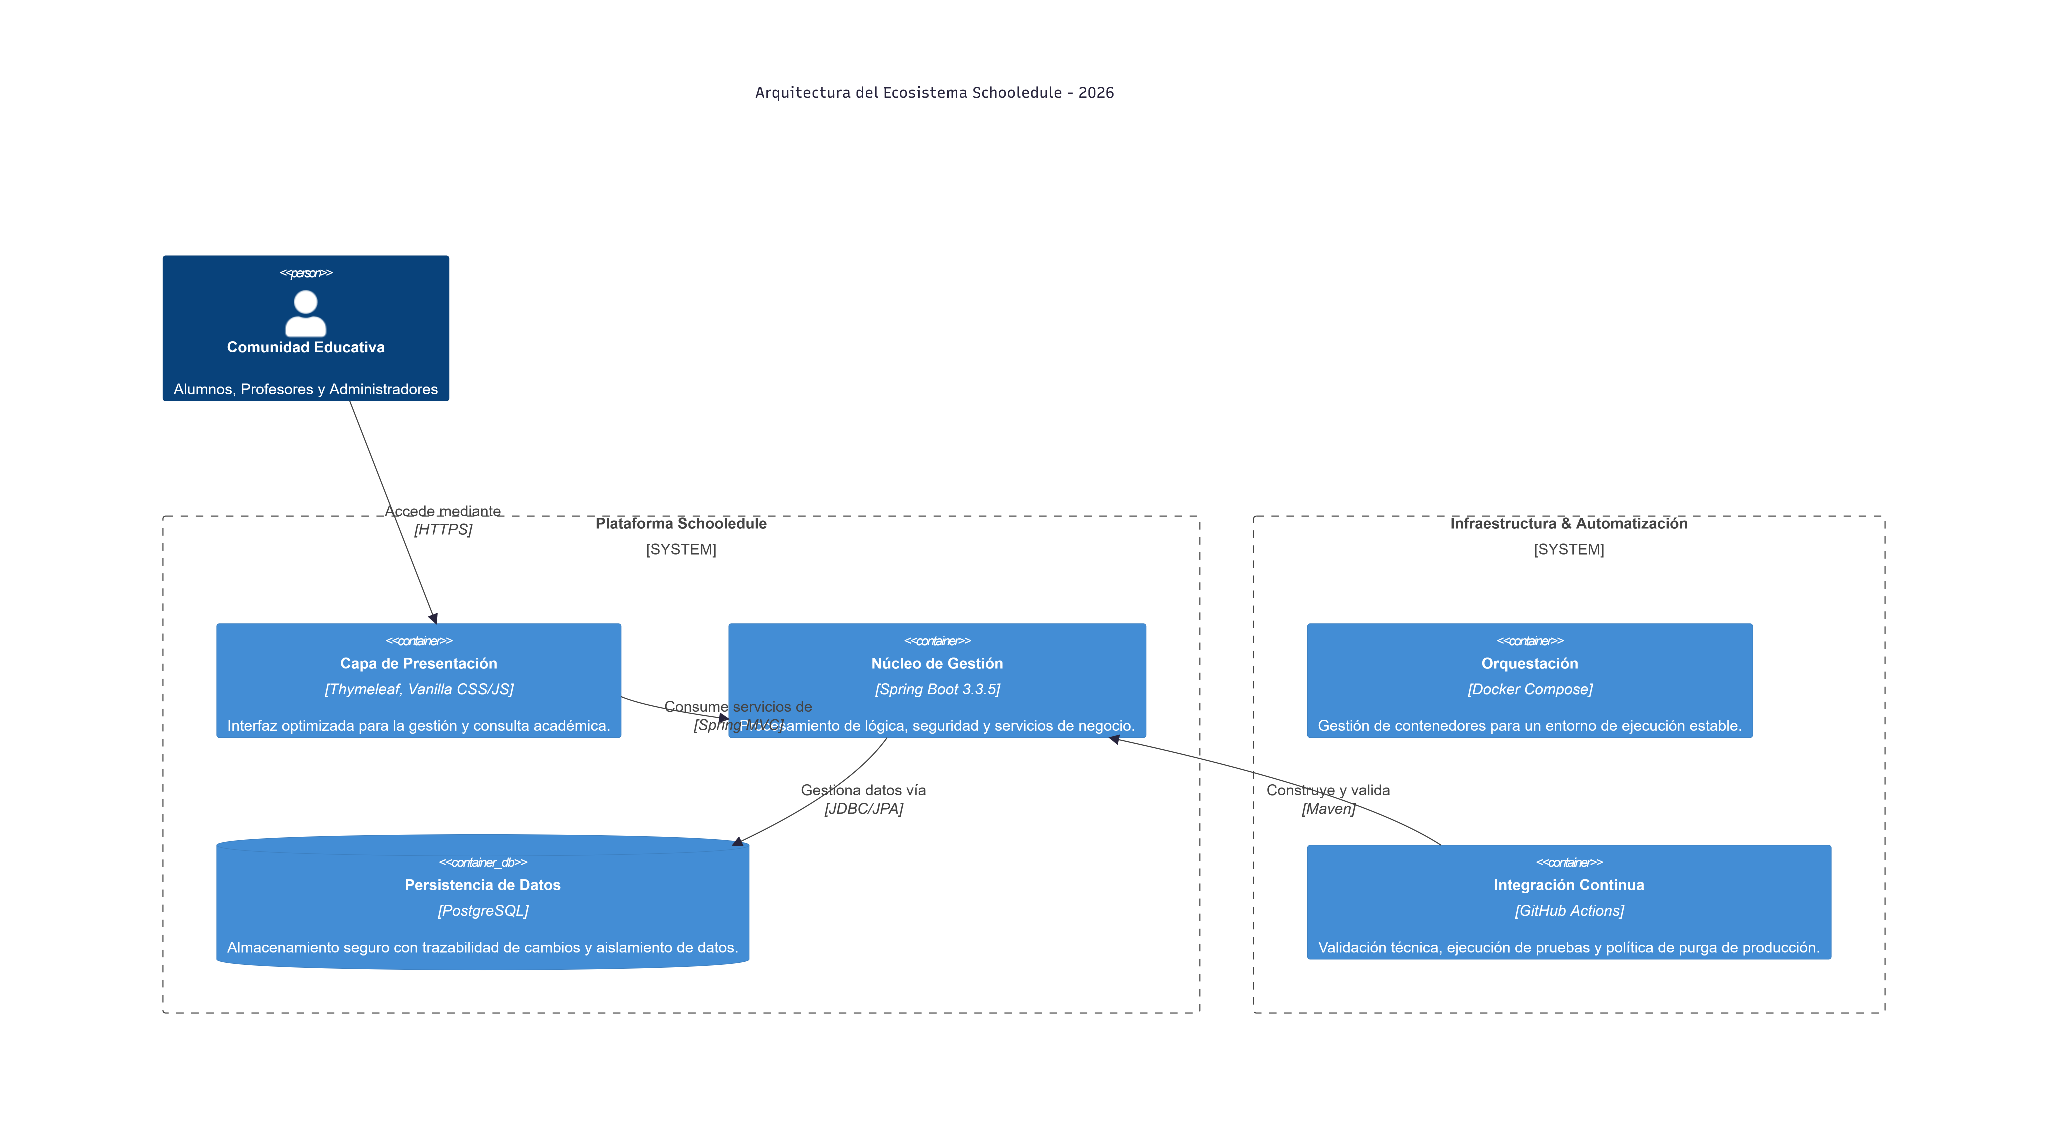
\includegraphics[width=\textwidth]{image10.png}
  \caption{Diagrama C4 -- Arquitectura del Ecosistema Schooledule}
  \label{fig:arquitectura-c4}
\end{figure}

\begin{enumerate}
  \item \textbf{Capa de Presentación (Interfaz de Usuario):} Se ha optado por una combinación de Thymeleaf con Vanilla CSS y JavaScript. Esta elección busca minimizar la carga en el cliente y garantizar una respuesta rápida del sistema, proporcionando una interfaz limpia y profesional que facilite la gestión de notas y perfiles.

  \item \textbf{Capa de Lógica de Negocio (Servidor):} El núcleo de la aplicación está desarrollado con Spring Boot 3.3.5 y Java 21. Esta capa orquesta todas las reglas académicas, desde la gestión de matrículas hasta la validación de roles (RBAC), apoyándose en Spring Data JPA y Spring MVC.

  \item \textbf{Capa de Datos (Persistencia):} La base de datos PostgreSQL actúa como el pilar de integridad. Se ha implementado un sistema de Auditoría Forense que registra cualquier modificación en las calificaciones, asegurando que el historial académico sea fiable y auditable en todo momento.
\end{enumerate}

\section{Ciclo de Calidad y Gestión del Proyecto}

Para asegurar que la entrega final sea impecable y profesional, se ha dise\~nado un flujo de automatización en GitHub Actions dividido en cuatro fases críticas:

\begin{figure}[H]
  \centering
  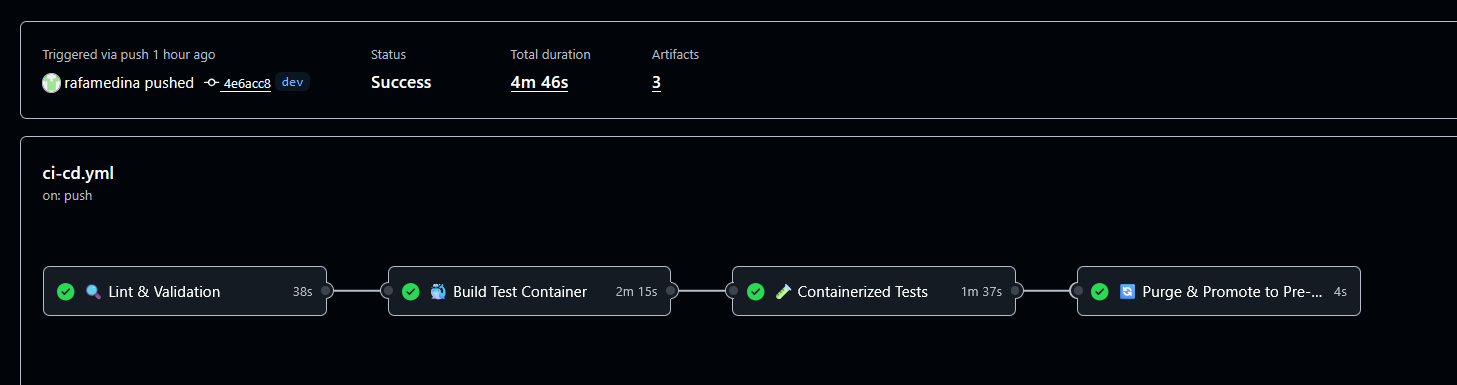
\includegraphics[width=\textwidth]{image17.png}
  \caption{Pipeline CI/CD en GitHub Actions -- ejecución real del flujo de automatización}
  \label{fig:pipeline-cicd}
\end{figure}

\begin{itemize}
  \item \textbf{Validación y Estilo (Linting):} Antes de procesar el código, el sistema audita cada línea. Se han configurado herramientas que verifican el estilo del código Java (Spotless), la seguridad del Dockerfile (Hadolint) y la sintaxis de las configuraciones.

  \item \textbf{Construcción en Contenedor (Build):} La aplicación se compila dentro de una imagen Docker aislada, garantizando que el binario resultante sea idéntico independientemente del entorno.

  \item \textbf{Pruebas Reales (Test \& Quality Gate):} El sistema levanta una base de datos PostgreSQL real y ejecuta todas las pruebas unitarias e integrales dentro de un contenedor. El despliegue se bloquea automáticamente si la cobertura de código (JaCoCo) no supera el 80\%.

  \item \textbf{Purga y Promoción (Purge Policy):} Una vez validado el código, el sistema crea automáticamente una versión de producción eliminando todas las herramientas de soporte internas. El flujo es:
    \begin{enumerate}
      \item Se crea la nueva función en la rama \texttt{dev}.
      \item Si el push pasa todas las pruebas, se limpia el repositorio.
      \item Se crea una rama \texttt{pre-prod}.
      \item Se genera automáticamente una pull request a \texttt{main}.
    \end{enumerate}
\end{itemize}

\section{Casos de Uso}

Los cuatro actores del sistema son:

\begin{enumerate}
  \item \textbf{Alumno:} Usuario final que consulta su progreso académico, calificaciones y perfil personal.
  \item \textbf{Profesor:} Responsable de la gestión académica de sus módulos y de la evaluación de los alumnos matriculados. Los profesores asignados como tutores de grupo acceden adicionalmente a la vista de seguimiento del tutor.
  \item \textbf{Administrador de Centro:} Gestor delegado con alcance limitado a los centros que tiene asignados: gestiona grupos, imparticiones, matrículas y usuarios sin privilegios de administración global.
  \item \textbf{Administrador Global:} Perfil con privilegios completos sobre toda la infraestructura del sistema: centros, usuarios, módulos, cursos académicos, grupos, imparticiones, alumnos y auditoría.
\end{enumerate}

\begin{figure}[H]
  \centering
  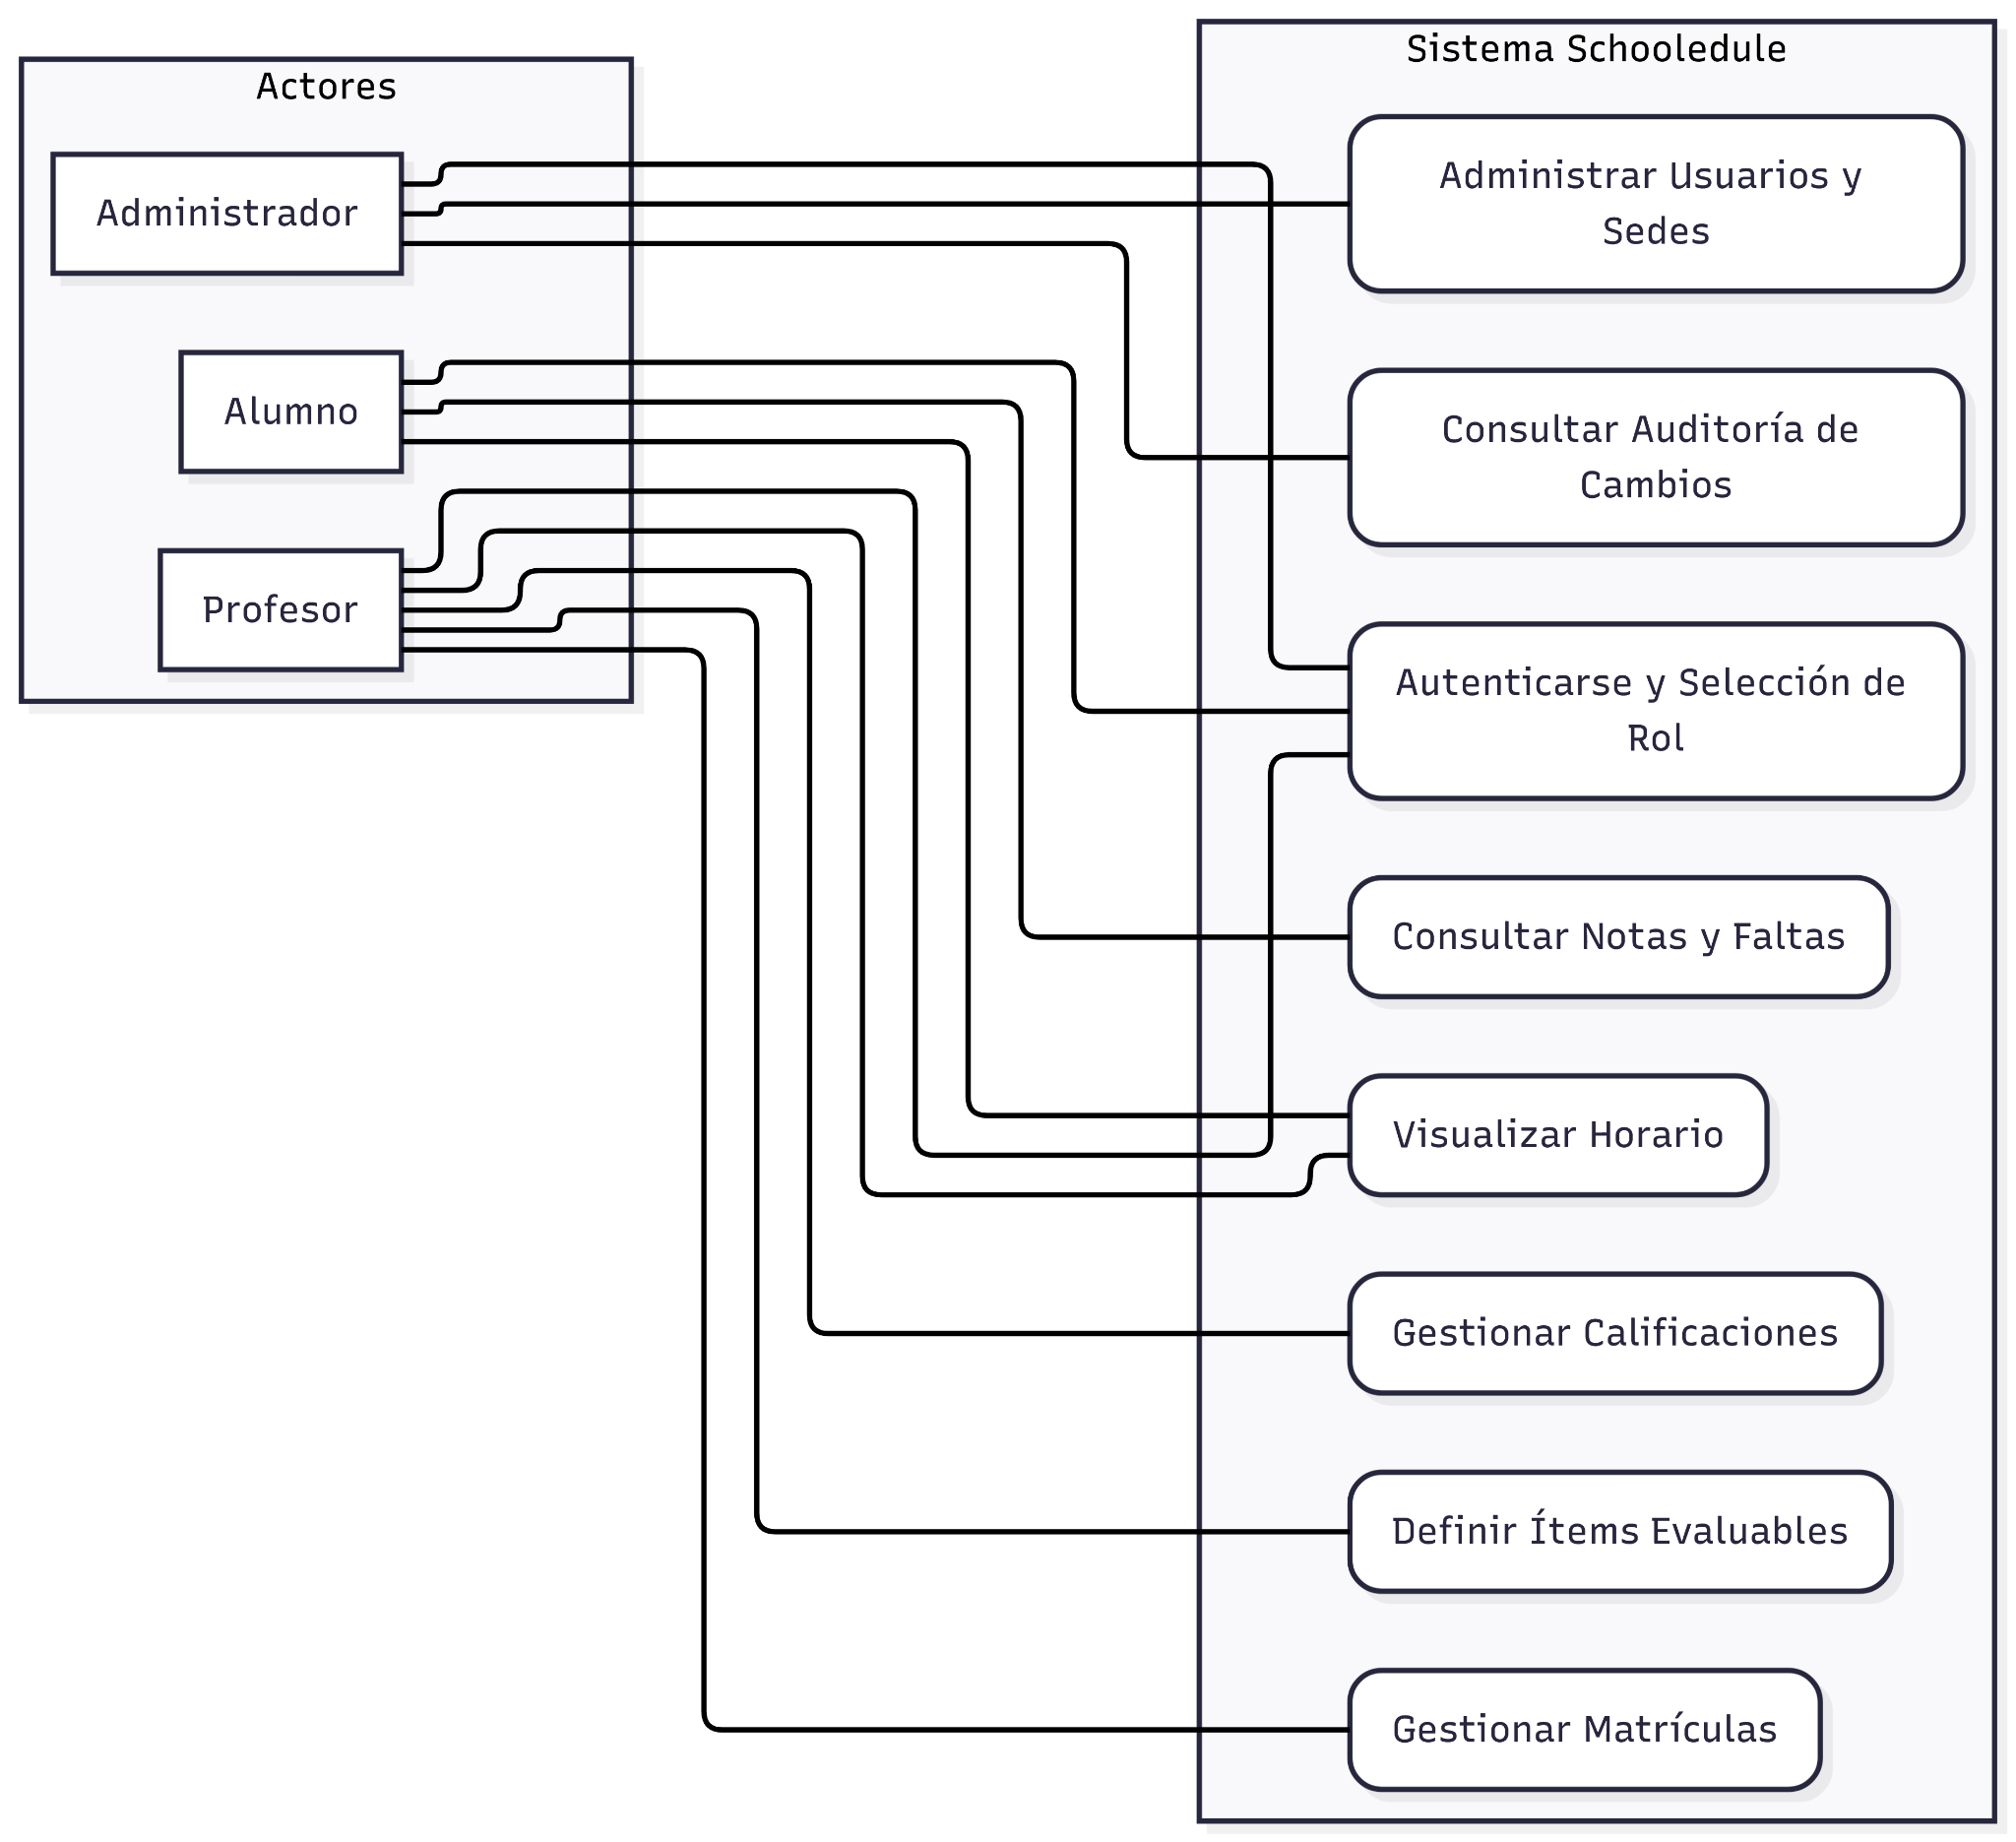
\includegraphics[width=0.85\textwidth]{image13.png}
  \caption{Diagrama de Casos de Uso del Sistema Schooledule}
  \label{fig:casos-uso}
\end{figure}

\subsection{Descripción de los Casos de Uso Principales}

\subsubsection{Gestión de Identidad y Acceso}
\begin{itemize}
  \item \textbf{Autenticarse y Selección de Rol:} Todos los usuarios deben identificarse. Dado que un usuario puede tener múltiples roles, el sistema permite seleccionar el perfil activo al iniciar la sesión.
\end{itemize}

\subsubsection{Interacciones del Alumnado}
\begin{itemize}
  \item \textbf{Consultar Notas:} Acceso a las calificaciones obtenidas en los diferentes criterios de evaluación y resultados de aprendizaje, desglosadas por período.
\end{itemize}

\subsubsection{Gestión Docente}
\begin{itemize}
  \item \textbf{Gestionar Calificaciones:} El profesor puede introducir y modificar notas, sujetas al sistema de auditoría.
  \item \textbf{Definir ítems Evaluables:} Configuración de las actividades y criterios que componen la evaluación de un módulo.
\end{itemize}

\subsubsection{Administración y Control}
\begin{itemize}
  \item \textbf{Administrar Usuarios y Sedes:} Gestión de altas, bajas y asignación de centros a través del sistema multi-sede.
  \item \textbf{Consultar Auditoría:} Herramienta crítica para rastrear quién, cuándo y por qué se modificó una calificación.
\end{itemize}

\section{Diagrama de Clases}

El modelo de dominio se ha dise\~nado siguiendo principios de Dise\~no Orientado al Dominio (DDD), asegurando que cada clase tenga una responsabilidad clara y coherente con las reglas académicas.

\begin{figure}[H]
  \centering
  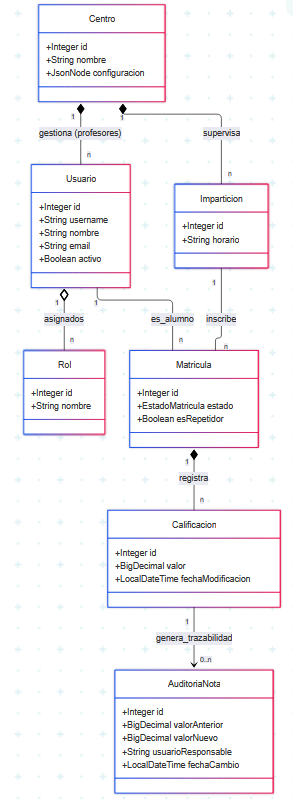
\includegraphics[width=0.6\textwidth]{image7.png}
  \caption{Diagrama de Clases del dominio de Schooledule}
  \label{fig:diagrama-clases}
\end{figure}

\subsection{Gestión de Usuarios y Seguridad}
\begin{itemize}
  \item \textbf{Usuario:} Clase central que representa a cualquier persona que accede al sistema.
  \item \textbf{Rol:} Define los permisos y capacidades de un usuario. La relación es N:M (gestionada por una tabla intermedia), permitiendo la polivalencia de perfiles.
\end{itemize}

\subsection{Estructura Organizativa}
\begin{itemize}
  \item \textbf{Centro:} Representa la sede física y lógica. Es el eje del aislamiento de datos (multi-sede).
  \item \textbf{Grupo:} Agrupación de alumnos en un curso y a\~no académico específico.
\end{itemize}

\subsection{Proceso Académico}
\begin{itemize}
  \item \textbf{Matrícula:} Vincula a un alumno con una impartición específica en un centro. Gestiona el estado académico (activo, baja, etc.).
  \item \textbf{Calificación:} Almacena el resultado numérico de un ítem evaluable para una matrícula concreta.
  \item \textbf{AuditoriaNota:} Clase especializada en la trazabilidad inmutable de cualquier cambio realizado en una calificación.
\end{itemize}

\subsection{Relaciones y Lógica de Negocio}
\begin{itemize}
  \item \textbf{Composición o Agregación:} Se ha utilizado composición en casos donde la vida de la entidad secundaria depende estrictamente de la principal.
  \item \textbf{Trazabilidad Inmutable:} La relación entre \texttt{Calificacion} y \texttt{AuditoriaNota} es unidireccional. La auditoría nunca se modifica; solo se crean nuevos registros ante cambios en la calificación.
  \item \textbf{Aislamiento Multi-Sede:} La relación con \texttt{Centro} es transversal a todas las operaciones de persistencia.
\end{itemize}

\section{Diagrama E/R (Entidad-Relación)}

\begin{figure}[H]
  \centering
  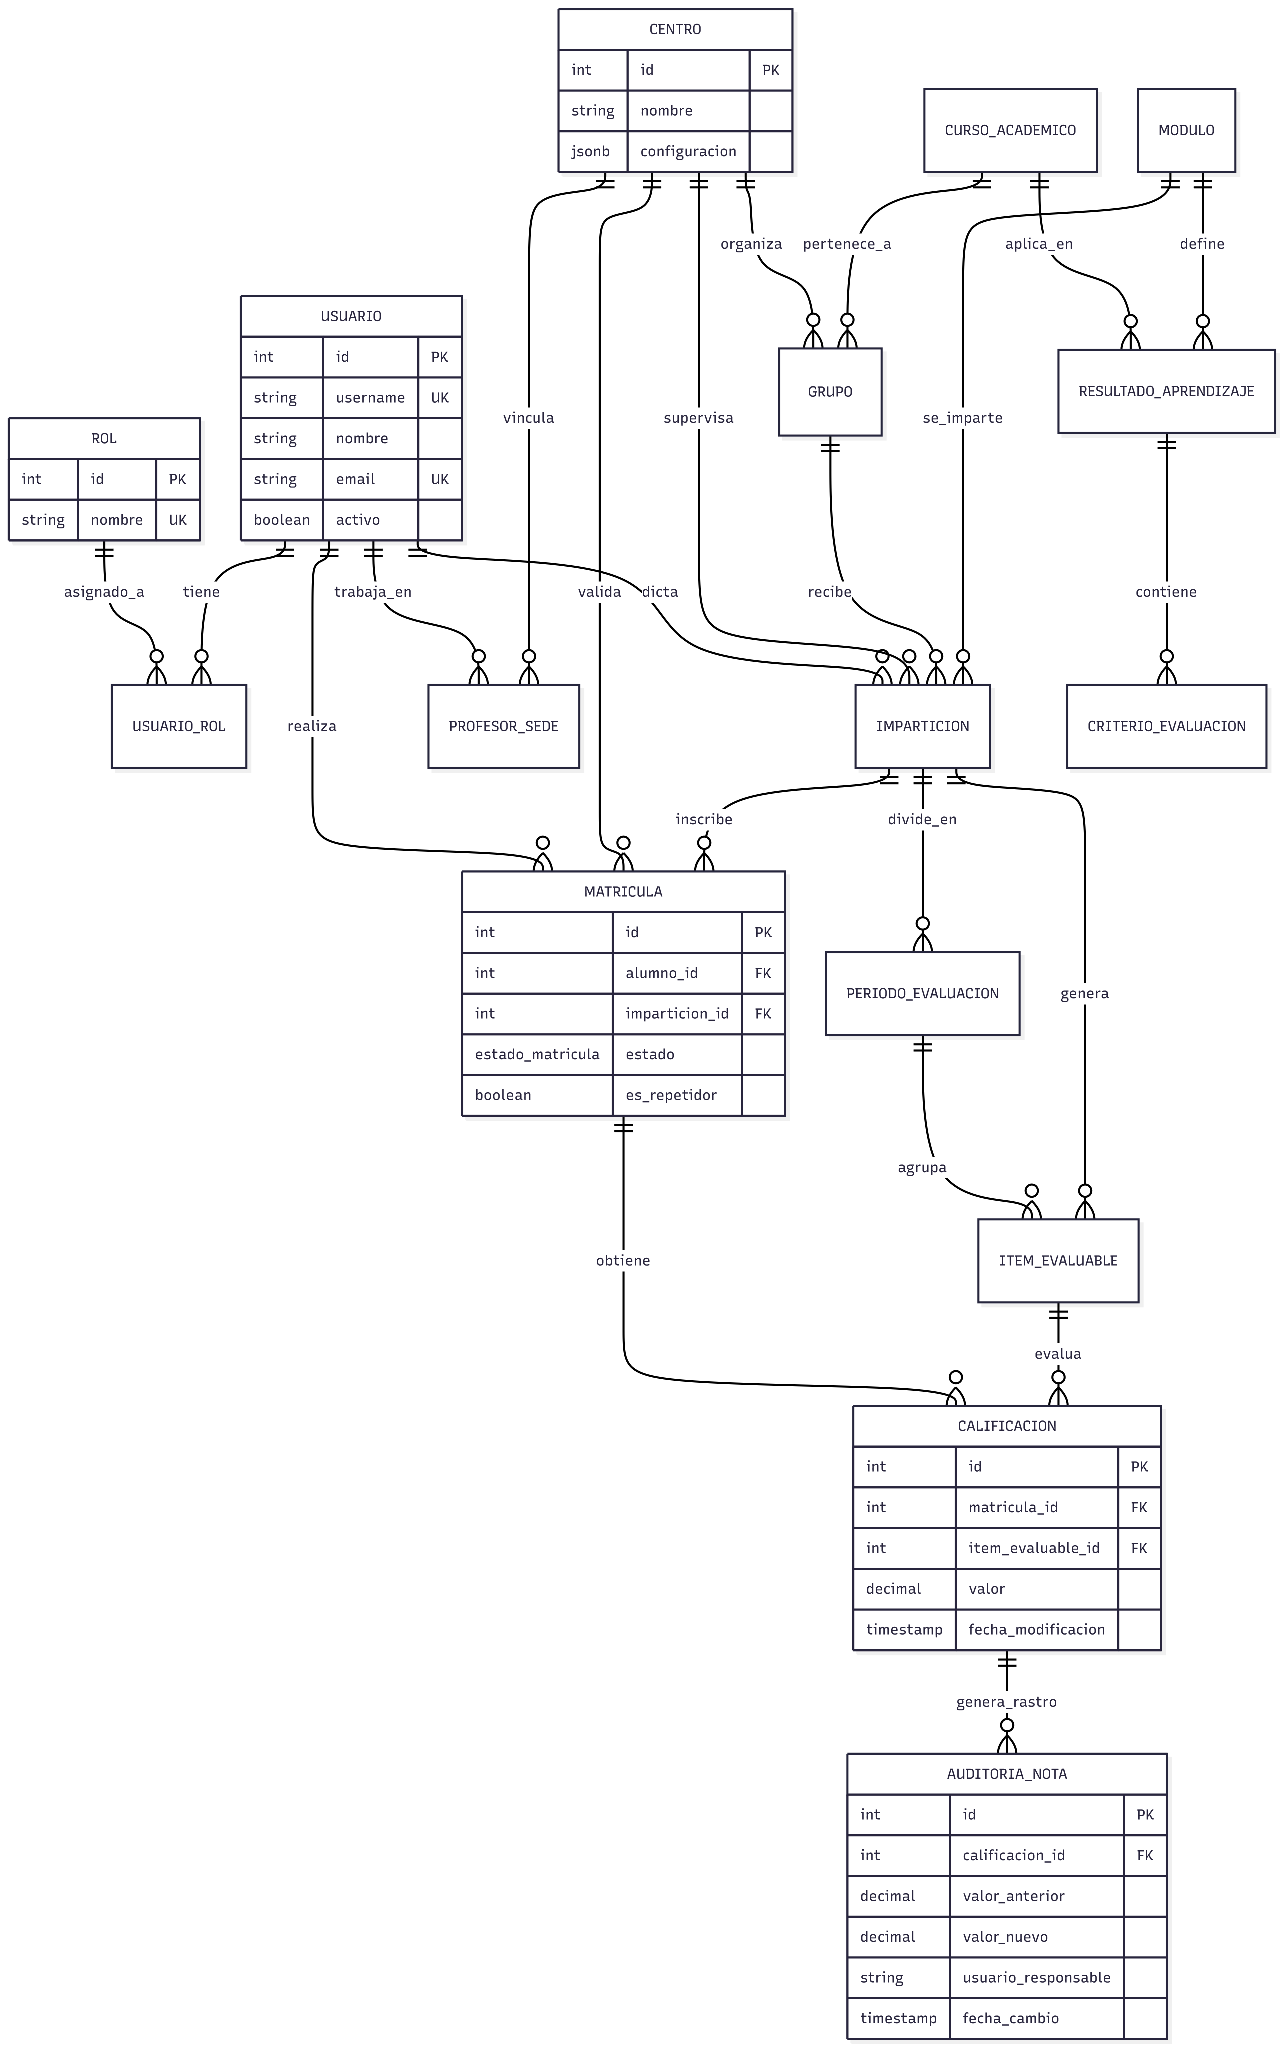
\includegraphics[width=0.88\textwidth]{image6.png}
  \caption{Diagrama Entidad-Relación completo de Schooledule}
  \label{fig:diagrama-er}
\end{figure}

\subsection{Configuración Curricular y Académica}
\begin{itemize}
  \item \textbf{MóDULO y RESULTADO\_APRENDIZAJE:} Los módulos definen los objetivos pedagógicos a través de resultados de aprendizaje, los cuales se desglosan en \textbf{CRITERIO\_EVALUACION}. Esta estructura permite una evaluación competencial detallada.
  \item \textbf{CURSO\_ACADEMICO:} Actúa como un eje temporal, permitiendo que la configuración curricular evolucione entre a\~nos sin perder el histórico de datos.
\end{itemize}

\subsection{El Nodo Central: La Impartición}

La entidad \textbf{IMPARTICIóN} es el pivot fundamental del sistema. Vincula cuatro dimensiones críticas:
\begin{itemize}
  \item \textbf{Qué:} El Módulo profesional.
  \item \textbf{Quién:} El Usuario (Profesor) que dicta la materia.
  \item \textbf{A quién:} El Grupo de alumnos que recibe la formación.
  \item \textbf{Dónde:} El Centro educativo que supervisa la actividad.
\end{itemize}

\subsection{Gestión de Matrícula y Aislamiento de Sedes}
\begin{itemize}
  \item \textbf{Multi-Tenencia:} La entidad \textbf{CENTRO} es la raíz de la seguridad. Mediante relaciones directas con \texttt{GRUPO}, \texttt{IMPARTICIóN} y \texttt{MATRICULA}, el sistema garantiza que un usuario solo pueda acceder a los registros del centro donde tiene permisos activos.
  \item \textbf{Estado de la Matrícula:} La entidad \textbf{MATRICULA} permite rastrear la situación del alumno mediante el enumerado \texttt{estado\_matricula} con los valores \texttt{ACTIVA}, \texttt{BAJA} y \texttt{CONVALIDADO}, y si el alumno es repetidor.
\end{itemize}

\subsection{Ciclo de Evaluación y Auditoría Forense}
\begin{itemize}
  \item \textbf{ITEM\_EVALUABLE:} Representa cualquier actividad evaluativa (exámenes, proyectos, etc.) asociada a una impartición y un periodo de evaluación concreto.
  \item \textbf{AUDITORIA\_NOTA:} Es el componente de integridad crítica. Ante cualquier actualización de la tabla \texttt{CALIFICACIóN}, se dispara una inserción obligatoria en esta tabla. Se registra el valor previo, el nuevo, la fecha exacta y el usuario responsable.
\end{itemize}

\subsection{Identidad y Roles N:M}

La relación entre \textbf{USUARIO} y \textbf{ROL} mediante la tabla intermedia \texttt{usuarios\_roles} elimina la rigidez de los perfiles únicos. Un usuario puede actuar como ``Profesor'' en una impartición y como ``Administrador'' de su sede simultáneamente.

%=============================================================
% CAPITULO 6 - TECNOLOGIA
%=============================================================
\chapter{Tecnología}

A continuación se describen las tecnologías y herramientas utilizadas en el proyecto.

\begin{longtable}{>{\centering\arraybackslash}p{2cm} >{\bfseries}p{2.8cm} p{4.4cm} p{4.4cm}}
  \toprule
  \textbf{Logo} & \textbf{Herramienta} & \textbf{Descripción} & \textbf{Uso en el proyecto} \\
  \midrule
  \endfirsthead
  \toprule
  \textbf{Logo} & \textbf{Herramienta} & \textbf{Descripción} & \textbf{Uso en el proyecto} \\
  \midrule
  \endhead
  \bottomrule
  \endfoot

  \logo{image4.png} & Java 21
    & Lenguaje de programación robusto y multiplataforma con soporte nativo para características modernas de alto rendimiento.
    & Base fundamental para la implementación de la lógica de negocio, servicios del backend y gestión de la concurrencia. \\[8pt]

  \logo{image18.png} & Spring Boot 3.3.5
    & Framework de código abierto dise\~nado para simplificar el arranque y desarrollo de aplicaciones Java empresariales.
    & Orquestador central de la aplicación, gestionando la inyección de dependencias, la seguridad (RBAC) y los servicios web. \\[8pt]

  \logo{image9.png} & Thymeleaf
    & Motor de plantillas Java moderno que permite procesar HTML, XML y otros formatos en el lado del servidor.
    & Generación dinámica de la capa de presentación y visualización de datos académicos para los diferentes perfiles de usuario. \\[8pt]

  \logo{image2.png} & PostgreSQL 16
    & Sistema de gestión de bases de datos relacionales potente y extensible con soporte avanzado para JSONB y auditoría.
    & Almacenamiento persistente de datos académicos, perfiles de usuario y rastro inmutable de calificaciones. \\[8pt]

  \logo{image8.png} & Flyway
    & Herramienta de control de versiones para bases de datos que automatiza la aplicación de cambios en el esquema SQL.
    & Gestión de migraciones y mantenimiento de la coherencia estructural de la base de datos en todos los entornos. \\[8pt]

  \logo{image15.png} & Docker \& Compose
    & Plataforma de contenedores que permite empaquetar aplicaciones y sus dependencias en entornos aislados y portables.
    & Garantía de paridad entre entornos mediante la orquestación de servicios y la base de datos en contenedores. \\[8pt]

  \logo{image3.png} & GitHub Actions
    & Plataforma de automatización de flujos de trabajo integrada en el ecosistema de control de versiones de GitHub.
    & Ejecución del pipeline de CI/CD, validación de calidad de código y automatización del despliegue en producción. \\[8pt]

  \logo{image14.png} & Maven
    & Herramienta de automatización de construcción que gestiona el ciclo de vida del proyecto y sus dependencias externas.
    & Estandarización del proceso de compilación, gestión de librerías y ejecución de las baterías de pruebas. \\[8pt]

  \logo{image11.png} & JUnit 5 \& Mockito
    & Frameworks líderes para la realización de pruebas unitarias y simulaciones de comportamiento en aplicaciones Java.
    & Implementación de la estrategia de pruebas para validar la lógica de negocio y asegurar la integridad del software. \\[8pt]

  \logo{image1.png} & JaCoCo
    & Librería de código abierto para medir la cobertura de código en proyectos Java durante la ejecución de pruebas.
    & Monitorización del porcentaje de código validado para asegurar el cumplimiento del estándar de calidad del 80\%. \\[8pt]

  & Bucket4j
    & Librería Java de limitación de tasa basada en el algoritmo \textit{token bucket}, compatible con almacenamiento en memoria y distribuido.
    & Implementación del filtro \texttt{LoginRateLimitFilter} que restringe los intentos de autenticación a 10 por dirección IP cada 15 minutos, retornando HTTP 429 al superarse el límite. \\[8pt]

  \logo{image9.png} & pre-commit
    & Marco de trabajo para la gestión y ejecución de ganchos (hooks) antes de confirmar cambios en el control de versiones.
    & Automatización de la validación de código en el entorno local para prevenir errores antes del commit. \\[8pt]

  \logo{image5.png} & Prettier
    & Formateador de código con soporte para múltiples lenguajes que garantiza un estilo consistente en archivos de frontend.
    & Estandarización del formato en archivos CSS, JavaScript, HTML, YAML y Markdown. \\[8pt]

  \logo{image16.png} & Spotless
    & Plugin de formateo de código para proyectos Java que aplica estándares consistentes de legibilidad.
    & Mantenimiento automático del estilo de código de Google en todos los archivos fuente de Java. \\

\end{longtable}

%=============================================================
% CAPITULOS POR COMPLETAR
%=============================================================

\chapter{Análisis de Requisitos}

A continuación se presenta el desglose RFTP (\textbf{R}equisitos, \textbf{F}unciones, \textbf{T}areas y \textbf{P}ruebas) de las funcionalidades implementadas hasta la fecha. Cada requisito expresa en lenguaje coloquial lo que el sistema debe lograr; sus funciones lo desglosan en términos técnicos; las tareas describen el alcance concreto de cada desarrollo; y las pruebas planificadas demuestran que cada tarea ha sido completada satisfactoriamente, siguiendo la metodología TDD.

%-------------------------------------------------------------
\section{R01 -- El sistema debe permitir el acceso únicamente a usuarios registrados con credenciales válidas}

La plataforma no puede ser accesible de forma anónima. Cualquier operación académica (consultar notas, gestionar calificaciones, administrar centros) requiere que el usuario se haya identificado previamente con sus datos personales.

\subsection{R01F01 -- El usuario debe existir en el sistema con sus datos almacenados de forma segura}

El almacenamiento de identidades se realiza sobre PostgreSQL aplicando un esquema RBAC. Las contraseñas se guardan siempre cifradas mediante BCrypt, nunca en texto plano.

\subsubsection{R01F01T01 -- Crear la tabla \texttt{usuarios} en la base de datos}
Diseñar y aplicar mediante Flyway (migración V1) la tabla \texttt{usuarios} con los campos: \texttt{id}, \texttt{username}, \texttt{password\_hash}, \texttt{nombre}, \texttt{apellidos}, \texttt{email}, \texttt{activo} y \texttt{fecha\_registro}. Incluir las restricciones de unicidad sobre \texttt{username} y \texttt{email}.
\begin{itemize}
  \item \textbf{R01F01T01P01 --} Ejecutar la migración V1 en un entorno limpio y verificar que la tabla \texttt{usuarios} se crea correctamente en PostgreSQL con todas sus restricciones.
\end{itemize}

\subsubsection{R01F01T02 -- Crear las tablas \texttt{roles} y \texttt{usuarios\_roles} para el control de acceso basado en roles (RBAC)}
Diseñar la tabla \texttt{roles} con los cuatro valores \texttt{ROLE\_ADMIN}, \texttt{ROLE\_ADMIN\_CENTRO}, \texttt{ROLE\_PROFESOR} y \texttt{ROLE\_ALUMNO}, y la tabla de unión \texttt{usuarios\_roles} que implementa la relación N:M entre usuarios y roles.
\begin{itemize}
  \item \textbf{R01F01T02P01 --} Insertar un usuario de prueba con rol \texttt{PROFESOR} y confirmar que el registro aparece correctamente en la tabla \texttt{usuarios\_roles}.
\end{itemize}

\subsubsection{R01F01T03 -- Implementar \texttt{CustomUserDetailsService} para la integración con Spring Security}
Crear el servicio que implementa \texttt{UserDetailsService} de Spring Security, cargando al usuario por email desde la base de datos y construyendo el objeto \texttt{UserDetails} con sus roles como \texttt{GrantedAuthority}.
\begin{itemize}
  \item \textbf{R01F01T03P01 --} Intentar el inicio de sesión con un email inexistente y verificar que Spring Security lanza \texttt{UsernameNotFoundException} con respuesta HTTP 401.
\end{itemize}

\subsection{R01F02 -- El usuario debe introducir su email y contraseña para poder acceder}

La autenticación se realiza mediante un formulario HTML estándar procesado por Spring Security, con cifrado BCrypt para la verificación de contraseñas.

\subsubsection{R01F02T01 -- Diseñar la pantalla \texttt{login.html} con los campos de acceso}
Crear la vista Thymeleaf con los campos de email y contraseña, el botón de acceso y los mensajes de error para credenciales inválidas o sesión cerrada.
\begin{itemize}
  \item \textbf{R01F02T01P01 --} Acceder a \texttt{/login} sin sesión iniciada y confirmar que el formulario se renderiza correctamente sin requerir autenticación previa.
\end{itemize}

\subsubsection{R01F02T02 -- Configurar \texttt{SecurityConfig} para procesar el login en \texttt{/login}}
Definir el \texttt{SecurityFilterChain} con \texttt{loginProcessingUrl("/login")}, proteger las rutas por rol (\texttt{/admin/**} para ADMIN, \texttt{/centro-admin/**} para ADMIN\_CENTRO, \texttt{/profe/**} y \texttt{/tutor/**} para PROFESOR, \texttt{/alumno/**} para ALUMNO) y configurar el cierre de sesión en \texttt{/logout}.
\begin{itemize}
  \item \textbf{R01F02T02P01 --} Enviar credenciales correctas al endpoint \texttt{/login} y comprobar que la sesión HTTP se establece y redirige al panel correspondiente.
\end{itemize}

\subsubsection{R01F02T03 -- Aplicar cifrado BCrypt para el almacenamiento y verificación de contraseñas}
Registrar el bean \texttt{BCryptPasswordEncoder} en \texttt{SecurityConfig} y utilizarlo en \texttt{UsuarioService} para codificar las contraseñas antes de persistirlas.
\begin{itemize}
  \item \textbf{R01F02T03P01 --} Verificar que el valor almacenado en el campo \texttt{password\_hash} de la base de datos no coincide en texto plano con la contraseña original introducida.
\end{itemize}

\subsection{R01F03 -- Tras el login exitoso, el usuario debe ser redirigido al panel correspondiente a su rol}

Dado que un usuario puede tener múltiples roles funcionales, el sistema determina automáticamente el destino de la redirección o presenta una pantalla de selección cuando hay ambigüedad.

\subsubsection{R01F03T01 -- Implementar \texttt{CustomLoginSuccessHandler} con lógica de redirección por rol}
Crear el componente que inspecciona las autoridades del objeto \texttt{Authentication} y redirige a \texttt{/admin/dashboard}, \texttt{/centro-admin/dashboard}, \texttt{/profe/dashboard} o \texttt{/alumno/dashboard} según el rol activo. Si el usuario tiene más de un rol funcional, redirigir a \texttt{/seleccionar-rol}. Si no tiene ningún rol válido, redirigir a \texttt{/login?norole}.
\begin{itemize}
  \item \textbf{R01F03T01P01 --} Iniciar sesión con un usuario de rol único \texttt{PROFESOR} y comprobar que la redirección aterriza directamente en \texttt{/profe/dashboard}.
\end{itemize}

\subsubsection{R01F03T02 -- Implementar la pantalla de selección de rol para usuarios con múltiples roles}
Crear la vista \texttt{seleccionar-rol.html} con los perfiles disponibles del usuario autenticado y la lógica de redirección al panel elegido.
\begin{itemize}
  \item \textbf{R01F03T02P01 --} Asignar dos roles funcionales a un usuario de prueba, iniciar sesión y verificar que el sistema presenta la pantalla de selección de rol antes de acceder a cualquier panel.
\end{itemize}

%-------------------------------------------------------------
\section{R02 -- El sistema debe aislar los datos entre distintos centros educativos}

La plataforma gestiona varios centros educativos desde una única instancia. Ningún usuario debe poder acceder a datos de un centro al que no pertenece, garantizando la privacidad entre sedes.

\subsection{R02F01 -- Cada centro educativo debe tener sus propios datos y usuarios vinculados}

La entidad \texttt{Centro} actúa como raíz de aislamiento. Toda la información académica (grupos, imparticiones, matrículas) está ligada a un centro concreto.

\subsubsection{R02F01T01 -- Crear la tabla \texttt{centros} en la base de datos}
Diseñar la tabla \texttt{centros} con los campos \texttt{id}, \texttt{nombre}, \texttt{ubicacion} y \texttt{configuracion} (tipo JSONB para parámetros flexibles por sede).
\begin{itemize}
  \item \textbf{R02F01T01P01 --} Insertar un centro de prueba y verificar que el campo \texttt{configuracion} acepta y persiste correctamente un objeto JSON arbitrario.
\end{itemize}

\subsubsection{R02F01T02 -- Crear la tabla \texttt{profesores\_sedes} para la asignación multi-sede}
Diseñar la tabla de unión que relaciona profesores con uno o varios centros, permitiendo que un mismo usuario imparta docencia en múltiples sedes sin duplicar su identidad.
\begin{itemize}
  \item \textbf{R02F01T02P01 --} Vincular un profesor a dos centros distintos y verificar que el servicio \texttt{getCentersForTeacher} devuelve ambos centros correctamente.
\end{itemize}

\subsection{R02F02 -- Las consultas académicas deben filtrarse siempre por el identificador de centro}

Toda consulta de datos académicos aplica un filtro implícito por \texttt{centro\_id} basado en la sesión del usuario autenticado, impidiendo el acceso cruzado entre sedes.

\subsubsection{R02F02T01 -- Implementar \texttt{ImparticionRepository} con filtrado por centro del profesor}
Crear las consultas JPQL/Spring Data que restringen las imparticiones devueltas al \texttt{centro\_id} sobre el que el profesor tiene permisos activos.
\begin{itemize}
  \item \textbf{R02F02T02P01 --} Autenticar un profesor y solicitar \texttt{/profe/centro/\{centroId\}/asignaturas}; verificar que únicamente se devuelven asignaturas de ese centro y que ninguna pertenece a otro centro no asignado.
\end{itemize}

%-------------------------------------------------------------
\section{R03 -- El profesor debe poder gestionar sus asignaturas y calificar a sus alumnos}

El portal del profesor es el núcleo operativo de la plataforma. Permite navegar desde los centros asignados hasta los alumnos individuales, y registrar calificaciones granulares con trazabilidad completa.

\subsection{R03F01 -- El profesor debe visualizar los centros a los que está asignado}

Al acceder al sistema, el profesor ve únicamente los centros donde tiene imparticiones activas, sin acceso a datos de otras sedes.

\subsubsection{R03F01T01 -- Implementar el endpoint \texttt{GET /profe/dashboard}}
Desarrollar en \texttt{ProfeController} el método que recupera los centros del profesor autenticado mediante \texttt{TeacherDashboardService.getCentersForTeacher} y los expone al modelo Thymeleaf.
\begin{itemize}
  \item \textbf{R03F01T01P01 --} Acceder a \texttt{/profe/dashboard} con sesión de profesor y confirmar que se listan exclusivamente los centros a los que dicho profesor está asignado.
\end{itemize}

\subsubsection{R03F01T02 -- Diseñar la vista \texttt{profe/dashboard.html} con los centros como tarjetas navegables}
Crear la plantilla Thymeleaf que renderiza cada centro como una tarjeta con nombre y enlace directo a su listado de asignaturas.
\begin{itemize}
  \item \textbf{R03F01T02P01 --} Verificar visualmente que cada tarjeta muestra el nombre del centro y que el enlace navega correctamente a \texttt{/profe/centro/\{centroId\}/asignaturas}.
\end{itemize}

\subsection{R03F02 -- El profesor debe visualizar las asignaturas que imparte en cada centro}

Desde un centro seleccionado, el profesor accede al listado de módulos que imparte, con información del grupo y del curso académico.

\subsubsection{R03F02T01 -- Implementar el endpoint \texttt{GET /profe/centro/\{centroId\}/asignaturas}}
Desarrollar en \texttt{ProfeController} el método que invoca \texttt{getSubjectsForTeacherAndCenter} y devuelve las imparticiones activas del profesor en ese centro.
\begin{itemize}
  \item \textbf{R03F02T01P01 --} Solicitar las asignaturas de un centro con un profesor que no tiene imparticiones en él y verificar que el sistema devuelve una lista vacía sin errores.
\end{itemize}

\subsubsection{R03F02T02 -- Diseñar la vista \texttt{profe/asignaturas.html}}
Crear la plantilla Thymeleaf que muestra el módulo, el grupo y el curso académico de cada impartición, con enlace al listado de alumnos.
\begin{itemize}
  \item \textbf{R03F02T02P01 --} Navegar desde el dashboard a un centro y comprobar que se renderizan correctamente las asignaturas con sus datos asociados.
\end{itemize}

\subsection{R03F03 -- El profesor debe ver el listado de alumnos matriculados en una impartición}

Desde una asignatura, el profesor accede a los alumnos con matrícula activa, pudiendo seleccionar a cada uno para consultar o editar sus calificaciones.

\subsubsection{R03F03T01 -- Implementar el endpoint \texttt{GET /profe/imparticion/\{imparticionId\}/alumnos}}
Desarrollar en \texttt{ProfeController} el método que invoca \texttt{getRosterForImparticion}, incluyendo validación de que el profesor tiene permiso sobre esa impartición.
\begin{itemize}
  \item \textbf{R03F03T01P01 --} Acceder al listado de alumnos de una impartición y verificar que únicamente aparecen alumnos con estado de matrícula \texttt{ACTIVA}.
\end{itemize}

\subsubsection{R03F03T02 -- Diseñar la vista \texttt{profe/alumnos.html}}
Crear la plantilla Thymeleaf que muestra nombre, apellidos e identificador de matrícula de cada alumno, con acceso al panel de notas.
\begin{itemize}
  \item \textbf{R03F03T02P01 --} Visualizar la pantalla de alumnos y comprobar que el nombre de la impartición aparece correctamente en el encabezado de la página.
\end{itemize}

\subsection{R03F04 -- El profesor debe poder consultar y registrar notas por criterio de evaluación}

La calificación es granular: cada nota se asigna a un \texttt{CriterioEvaluacion} concreto, que pertenece a un \texttt{ResultadoAprendizaje} dentro de un periodo de evaluación.

\subsubsection{R03F04T01 -- Crear la migración V3 que vincula ítems evaluables a resultados de aprendizaje y refactoriza \texttt{calificaciones}}
Diseñar y aplicar la migración Flyway V3 que: (1) inserta los datos de \texttt{resultados\_aprendizaje} y \texttt{criterios\_evaluacion} de los módulos del ciclo; (2) añade la columna \texttt{resultado\_aprendizaje\_id} a \texttt{items\_evaluables} con su restricción de clave foránea; y (3) sustituye la columna \texttt{item\_evaluable\_id} de \texttt{calificaciones} por \texttt{criterio\_evaluacion\_id}, eliminando la restricción de unicidad antigua y creando la nueva. Las tablas \texttt{resultados\_aprendizaje} y \texttt{criterios\_evaluacion} ya existen en el esquema de V1.
\begin{itemize}
  \item \textbf{R03F04T01P01 --} Aplicar la migración V3 y verificar que la restricción de clave foránea de \texttt{calificaciones} apunta a \texttt{criterios\_evaluacion} y que \texttt{items\_evaluables} tiene el campo \texttt{resultado\_aprendizaje\_id} poblado y con restricción \texttt{NOT NULL}.
\end{itemize}

\subsubsection{R03F04T02 -- Implementar \texttt{GET /profe/api/matricula/\{matriculaId\}/notas}}
Desarrollar el endpoint REST que devuelve el árbol completo de notas del alumno (periodos \(\rightarrow\) RA \(\rightarrow\) CE) en formato JSON mediante \texttt{TeacherDashboardService.getStudentGrades}.
\begin{itemize}
  \item \textbf{R03F04T02P01 --} Consultar las notas de una matrícula con datos reales y verificar que el JSON devuelto incluye los criterios de evaluación con sus valores numéricos.
\end{itemize}

\subsubsection{R03F04T03 -- Implementar \texttt{POST /profe/api/matricula/\{matriculaId\}/notas}}
Desarrollar el endpoint REST que persiste o actualiza calificaciones mediante \texttt{upsertGrades}, incluyendo validación de que el \texttt{matriculaId} del path coincide con el del cuerpo de la petición.
\begin{itemize}
  \item \textbf{R03F04T03P01 --} Enviar una nota nueva para un criterio de evaluación y verificar que el registro se persiste correctamente en la tabla \texttt{calificaciones}.
  \item \textbf{R03F04T03P02 --} Enviar la misma nota dos veces y verificar que la segunda operación actualiza el registro existente en lugar de crear uno duplicado.
\end{itemize}

\subsubsection{R03F04T04 -- Corregir la invisibilidad de ítems de tipo RECUPERACION en el modal de notas}
El servicio \texttt{TeacherDashboardService} construía un mapa \texttt{raId\,\textrightarrow\,ItemEvaluable} con un \textit{merge} que descartaba los ítems duplicados del mismo resultado de aprendizaje. Los ítems de tipo \texttt{RECUPERACION} compartían \texttt{raId} con el ítem principal y eran silenciosamente eliminados. La solución consiste en sustituir dicho mapa por una \texttt{List<ItemEvaluable>} agrupada por periodo, conservando todos los ítems como entradas independientes y ordenándolos: ítems ordinarios primero, recuperaciones a continuación.
\begin{itemize}
  \item \textbf{R03F04T04P01 --} Acceder al modal de calificación de un alumno con una recuperación registrada y verificar que tanto el ítem ordinario como el ítem RECUPERACION aparecen como bloques independientes dentro del mismo resultado de aprendizaje.
\end{itemize}

\subsubsection{R03F04T05 -- Añadir \texttt{itemEvaluableId} al DTO de guardado de notas}
Incorporar el campo \texttt{@NotNull @Positive Integer itemEvaluableId} al DTO interno \texttt{GradeUpsertRequest.Entry} para que el servicio identifique el ítem evaluable concreto y pueda aplicar sobre él las validaciones de periodo.
\begin{itemize}
  \item \textbf{R03F04T05P01 --} Enviar una petición de guardado con un \texttt{itemEvaluableId} inexistente y verificar que el servicio responde con HTTP 404.
\end{itemize}

\subsubsection{R03F04T06 -- Omitir la validación de periodo cerrado para ítems de tipo RECUPERACION}
En el método \texttt{upsertGrades} de \texttt{TeacherDashboardService}, si el ítem evaluable identificado es de tipo \texttt{RECUPERACION}, se omite la comprobación de si el periodo está cerrado, permitiendo registrar notas de recuperación independientemente del estado del periodo ordinario.
\begin{itemize}
  \item \textbf{R03F04T06P01 --} Intentar guardar una nota en un periodo cerrado usando un ítem ordinario y verificar que el sistema la rechaza. Repetir la misma operación con un ítem de tipo RECUPERACION y verificar que es aceptada correctamente.
\end{itemize}

\subsection{R03F05 -- El sistema debe registrar una auditoría inmutable de cada cambio en las calificaciones}

Cualquier modificación de una nota debe quedar registrada con el valor anterior, el valor nuevo, el responsable y la fecha exacta, garantizando la trazabilidad forense del expediente académico.

\subsubsection{R03F05T01 -- Crear la tabla \texttt{auditoria\_notas} y el trigger PL/pgSQL en la migración V1}
Diseñar la tabla con los campos \texttt{id}, \texttt{calificacion\_id} (FK a \texttt{calificaciones}), \texttt{valor\_anterior}, \texttt{valor\_nuevo}, \texttt{usuario\_responsable} y \texttt{fecha\_cambio}. Implementar la función \texttt{registrar\_cambio\_nota()} en PL/pgSQL y el trigger \texttt{trigger\_auditoria\_notas} que se dispara \texttt{AFTER UPDATE} sobre la tabla \texttt{calificaciones}, insertando un registro únicamente cuando el valor numérico cambia.
\begin{itemize}
  \item \textbf{R03F05T01P01 --} Actualizar el valor de una calificación existente y consultar \texttt{auditoria\_notas} verificando que se ha generado un registro con los valores anterior y nuevo correctos, y con el campo \texttt{usuario\_responsable} informado.
\end{itemize}

\subsubsection{R03F05T02 -- Propagar el usuario activo al trigger mediante \texttt{set\_config} en \texttt{upsertGrades}}
Dentro de la transacción de \texttt{upsertGrades} en \texttt{TeacherDashboardService}, ejecutar \texttt{SELECT set\_config('app.usuario\_actual', email, true)} antes de persistir las calificaciones, de modo que la función PL/pgSQL del trigger pueda leer el email del profesor y almacenarlo en \texttt{usuario\_responsable}.
\begin{itemize}
  \item \textbf{R03F05T02P01 --} Modificar una calificación desde el endpoint del profesor y consultar \texttt{auditoria\_notas} para confirmar que el campo \texttt{usuario\_responsable} contiene el email del profesor autenticado y no el usuario de base de datos del sistema.
\end{itemize}

%-------------------------------------------------------------
\section{R04 -- El alumno debe poder consultar su información académica y sus calificaciones}

El portal del alumno ofrece acceso de solo lectura al expediente personal: datos de perfil, matrículas activas y calificaciones organizadas por periodo de evaluación.

\subsection{R04F01 -- El alumno debe disponer de un menú de navegación principal}

Tras el inicio de sesión, el alumno accede a un menú que centraliza las secciones disponibles en su portal.

\subsubsection{R04F01T01 -- Implementar el endpoint \texttt{GET /alumno/dashboard} y la vista \texttt{alumno/menuAlumno.html}}
Crear el controlador \texttt{AlumnoController} con el método que devuelve la vista del menú principal del alumno, listando las opciones de perfil, notas y otras funcionalidades disponibles.
\begin{itemize}
  \item \textbf{R04F01T01P01 --} Acceder a \texttt{/alumno/dashboard} con sesión de alumno y verificar que el menú se renderiza sin errores y que las opciones de navegación están disponibles.
\end{itemize}

\subsection{R04F02 -- El alumno debe poder consultar su perfil personal y académico}

La sección de perfil muestra los datos personales del alumno y su situación de matrícula actual, sin exponer campos internos del sistema.

\subsubsection{R04F02T01 -- Implementar el endpoint \texttt{GET /alumno/perfil}}
Desarrollar el método en \texttt{AlumnoController} que obtiene el \texttt{AlumnoProfileDTO} del usuario autenticado mediante \texttt{UsuarioService.getAlumnoProfile} y lo expone al modelo.
\begin{itemize}
  \item \textbf{R04F02T01P01 --} Acceder a \texttt{/alumno/perfil} y comprobar que se muestran correctamente el nombre, los apellidos y los datos de matrícula activos del alumno.
\end{itemize}

\subsubsection{R04F02T02 -- Diseñar la vista \texttt{alumno/perfil.html}}
Crear la plantilla Thymeleaf que renderiza los datos del perfil del alumno sin exponer campos sensibles como \texttt{password\_hash} ni identificadores internos de la base de datos.
\begin{itemize}
  \item \textbf{R04F02T02P01 --} Inspeccionar el HTML generado y confirmar que ningún campo sensible del sistema (contraseña, IDs internos) aparece visible en la respuesta.
\end{itemize}

\subsection{R04F03 -- El alumno debe poder consultar sus calificaciones organizadas por periodo de evaluación}

Las calificaciones se presentan agrupadas por periodo, mostrando la jerarquía de resultados de aprendizaje y criterios de evaluación de cada módulo.

\subsubsection{R04F03T01 -- Implementar el endpoint \texttt{GET /alumno/notas}}
Desarrollar el método en \texttt{AlumnoController} que carga los periodos de evaluación disponibles y el \texttt{GradeDashboardDTO} del periodo seleccionado (o el primero por defecto si no se especifica ninguno).
\begin{itemize}
  \item \textbf{R04F03T01P01 --} Acceder a \texttt{/alumno/notas} con un alumno que tiene calificaciones registradas y verificar que las notas aparecen correctamente agrupadas por periodo de evaluación.
\end{itemize}

\subsubsection{R04F03T02 -- Diseñar la vista \texttt{alumno/dashboard\_notas.html} con selector de periodo}
Crear la plantilla Thymeleaf con un selector de periodo de evaluación y una tabla que muestra las calificaciones por módulo y criterio, actualizándose al cambiar el periodo seleccionado.
\begin{itemize}
  \item \textbf{R04F03T02P01 --} Cambiar el periodo en el selector de la vista y verificar que la tabla de notas se actualiza correctamente mostrando los datos del nuevo periodo seleccionado.
\end{itemize}

%-------------------------------------------------------------
\section{R05 -- El administrador debe poder gestionar los usuarios del sistema}

El administrador dispone de un panel web completo para el ciclo de vida de los usuarios: alta, edición de datos personales y credenciales, asignación de roles y vinculación a centros educativos, y activación o desactivación de cuentas. Todas las operaciones están protegidas mediante autenticación y control de acceso basado en rol.

\subsection{R05F01 -- El administrador debe poder visualizar la lista de usuarios ordenada}

El listado centraliza todos los usuarios del sistema, mostrando nombre, apellidos, email, estado de activación, roles asignados y centros vinculados.

\subsubsection{R05F01T01 -- Implementar \texttt{GET /admin/usuarios} con \texttt{AdminUsuarioListDTO}}
Desarrollar en \texttt{AdminUsuarioController} el método que invoca \texttt{AdminUsuarioService.listarTodos()} y expone al modelo la lista de usuarios ordenada por apellidos y nombre ascendentes.
\begin{itemize}
  \item \textbf{R05F01T01P01 --} Acceder al listado y verificar que los registros aparecen ordenados correctamente y que cada fila refleja los roles y centros asociados.
\end{itemize}

\subsection{R05F02 -- El administrador debe poder crear nuevos usuarios con roles y centros asignados}

El formulario de alta permite especificar los datos de identidad del nuevo usuario, seleccionar sus roles (ADMIN, PROFESOR, ALUMNO) y vincularlo a los centros que correspondan. La contraseña se valida con la política de complejidad del sistema.

\subsubsection{R05F02T01 -- Diseñar el formulario \texttt{GET /admin/usuarios/nuevo}}
Crear la vista Thymeleaf con campos de nombre, apellidos, email, nombre de usuario, contraseña y selección múltiple de roles y centros. Aplicar anotaciones Bean Validation en \texttt{AdminUsuarioFormDTO}: \texttt{@NotBlank}, \texttt{@Email}, \texttt{@Size} y \texttt{@ValidPassword} en la contraseña.
\begin{itemize}
  \item \textbf{R05F02T01P01 --} Enviar el formulario con una contraseña que no cumple la política (sin mayúsculas, sin dígito o menos de 8 caracteres) y verificar que el sistema rechaza la operación mostrando el mensaje de error correspondiente.
\end{itemize}

\subsubsection{R05F02T02 -- Implementar \texttt{POST /admin/usuarios/nuevo} con patrón PRG}
Validar unicidad de \texttt{username} y \texttt{email} antes de persistir, cifrar la contraseña con BCrypt y redirigir al listado tras la creación exitosa.
\begin{itemize}
  \item \textbf{R05F02T02P01 --} Intentar crear un usuario con un email ya registrado en el sistema y confirmar que el formulario se re-renderiza con el error de unicidad sin persistir el registro duplicado.
\end{itemize}

\subsection{R05F03 -- El administrador debe poder editar los datos de un usuario existente}

La edición permite modificar datos personales, roles y centros. El campo contraseña es opcional: si se deja vacío, el sistema conserva el hash existente sin regenerarlo.

\subsubsection{R05F03T01 -- Implementar \texttt{GET} y \texttt{POST /admin/usuarios/\{id\}/editar}}
Cargar los datos actuales del usuario en el formulario y procesarlos aplicando las mismas validaciones de unicidad que en la creación, excluyendo al propio usuario de la comprobación de email y username duplicados.
\begin{itemize}
  \item \textbf{R05F03T01P01 --} Editar únicamente el nombre de un usuario sin introducir contraseña y confirmar que el hash almacenado en base de datos no se modifica.
\end{itemize}

\subsection{R05F04 -- El administrador debe poder activar o desactivar cuentas de usuario}

La desactivación impide el acceso al sistema sin eliminar el historial del usuario. El sistema protege contra la desactivación del último administrador activo para evitar el bloqueo total del panel.

\subsubsection{R05F04T01 -- Implementar \texttt{POST /admin/usuarios/\{id\}/toggle-activo}}
Invertir el estado del campo \texttt{activo} del usuario. Antes de desactivar, verificar mediante \texttt{countAdminsActivos()} que existe al menos otro usuario con rol ADMIN activo.
\begin{itemize}
  \item \textbf{R05F04T01P01 --} Intentar desactivar al único administrador activo del sistema y verificar que la operación es rechazada con un mensaje explicativo, manteniéndose el estado \texttt{activo=true}.
\end{itemize}

%-------------------------------------------------------------
\section{R06 -- El administrador debe poder gestionar los centros educativos}

El catálogo de centros es el eje del aislamiento de datos multi-sede. El administrador puede dar de alta nuevas sedes, editar su información y controlar su disponibilidad para nuevas imparticiones.

\subsection{R06F01 -- El administrador debe poder listar los centros registrados}

\subsubsection{R06F01T01 -- Implementar \texttt{GET /admin/centros}}
Mostrar la lista de centros con nombre, ubicación y estado de activación.
\begin{itemize}
  \item \textbf{R06F01T01P01 --} Acceder al listado y confirmar que se muestran correctamente el nombre, la ubicación y el estado de cada sede.
\end{itemize}

\subsection{R06F02 -- El administrador debe poder crear y editar centros}

\subsubsection{R06F02T01 -- Implementar los formularios de alta y edición con validaciones}
Aplicar \texttt{@NotBlank} en nombre y ubicación. El formulario de edición carga los datos del centro seleccionado.
\begin{itemize}
  \item \textbf{R06F02T01P01 --} Intentar crear un centro con nombre vacío y verificar que el sistema muestra el mensaje de validación correspondiente.
  \item \textbf{R06F02T01P02 --} Editar la ubicación de un centro existente y confirmar que el cambio persiste en base de datos.
\end{itemize}

\subsection{R06F03 -- El administrador debe poder activar o desactivar centros}

\subsubsection{R06F03T01 -- Implementar \texttt{POST /admin/centros/\{id\}/toggle-activo}}
Permitir la desactivación de sedes sin eliminar su historial de imparticiones y matrículas.
\begin{itemize}
  \item \textbf{R06F03T01P01 --} Desactivar un centro y verificar que deja de aparecer en los selectores de nuevas imparticiones.
\end{itemize}

%-------------------------------------------------------------
\section{R07 -- El administrador debe poder gestionar el catálogo de módulos}

Los módulos representan los contenidos curriculares del ciclo formativo. El administrador gestiona el catálogo global, pudiendo añadir nuevos módulos, modificar sus datos y controlar su disponibilidad para nuevas imparticiones.

\subsection{R07F01 -- El administrador debe poder listar y crear módulos}

\subsubsection{R07F01T01 -- Implementar \texttt{GET /admin/modulos} y el formulario de alta}
Mostrar la lista completa de módulos con nombre, horas lectivas y estado. Validar \texttt{@NotBlank} en nombre y \texttt{@Positive} en horas.
\begin{itemize}
  \item \textbf{R07F01T01P01 --} Intentar crear un módulo con un valor negativo en las horas lectivas y verificar el rechazo con el mensaje de validación correspondiente.
\end{itemize}

\subsection{R07F02 -- El administrador debe poder editar y desactivar módulos}

\subsubsection{R07F02T01 -- Implementar la edición y el \texttt{toggle-activo} de módulos}
Permitir la modificación de nombre y horas, y la desactivación sin afectar a las imparticiones históricas del módulo.
\begin{itemize}
  \item \textbf{R07F02T01P01 --} Desactivar un módulo y confirmar que no aparece disponible al crear una nueva impartición.
\end{itemize}

%-------------------------------------------------------------
\section{R08 -- El administrador debe poder gestionar los cursos académicos}

El curso académico actúa como eje temporal del sistema, permitiendo separar los datos de cada a\~no lectivo sin perder el histórico de periodos anteriores.

\subsection{R08F01 -- El administrador debe poder listar, crear y editar cursos académicos}

\subsubsection{R08F01T01 -- Implementar \texttt{GET /admin/cursos} y los formularios de gestión}
Mostrar la lista de cursos con nombre. Validar unicidad del nombre en la creación para evitar registros duplicados.
\begin{itemize}
  \item \textbf{R08F01T01P01 --} Crear un curso con un nombre ya existente y verificar que el sistema lo impide con el mensaje de error apropiado.
\end{itemize}

%-------------------------------------------------------------
\section{R09 -- El administrador debe poder gestionar los grupos de alumnos}

Los grupos vinculan a los alumnos con un centro y un curso académico concreto. El administrador gestiona su creación y actualización desde el panel.

\subsection{R09F01 -- El administrador debe poder listar, crear y editar grupos}

\subsubsection{R09F01T01 -- Implementar \texttt{GET /admin/grupos} y los formularios de gestión}
Mostrar el nombre del grupo, el centro al que pertenece y el curso académico correspondiente. Validar los campos obligatorios en el formulario de alta.
\begin{itemize}
  \item \textbf{R09F01T01P01 --} Intentar crear un grupo sin seleccionar centro y verificar el mensaje de error de validación.
  \item \textbf{R09F01T01P02 --} Editar el curso académico de un grupo existente y confirmar que el cambio persiste correctamente.
\end{itemize}

%-------------------------------------------------------------
\section{R10 -- El administrador debe poder gestionar las imparticiones}

La impartición es el pivot central del modelo de datos: vincula el módulo, el profesor, el grupo y el centro en un curso académico concreto. El administrador crea y actualiza estas asignaciones.

\subsection{R10F01 -- El administrador debe poder listar las imparticiones}

\subsubsection{R10F01T01 -- Implementar \texttt{GET /admin/imparticiones}}
Mostrar cada impartición con las cuatro dimensiones que la definen: módulo, grupo, profesor y centro.
\begin{itemize}
  \item \textbf{R10F01T01P01 --} Acceder al listado y comprobar que cada fila refleja correctamente las cuatro dimensiones de la impartición.
\end{itemize}

\subsection{R10F02 -- El administrador debe poder crear y editar imparticiones}

\subsubsection{R10F02T01 -- Implementar el formulario de alta con validación de unicidad}
Ofrecer selectores de módulo (solo activos), grupo, centro y profesor. Validar que la combinación módulo-grupo no está ya registrada en el mismo curso para evitar duplicados.
\begin{itemize}
  \item \textbf{R10F02T01P01 --} Intentar crear una impartición duplicada y verificar que el sistema la rechaza con un mensaje descriptivo.
  \item \textbf{R10F02T01P02 --} Editar el profesor asignado a una impartición y confirmar el cambio en el listado.
\end{itemize}

%-------------------------------------------------------------
\section{R11 -- El administrador debe poder gestionar los alumnos y sus matrículas}

El administrador puede consultar el listado de alumnos del sistema y gestionar sus matrículas en las imparticiones disponibles: alta, edición de estado y, cuando no existan calificaciones asociadas, baja.

\subsection{R11F01 -- El administrador debe poder listar los alumnos registrados}

\subsubsection{R11F01T01 -- Implementar \texttt{GET /admin/alumnos}}
Recuperar los usuarios con rol \texttt{ROLE\_ALUMNO} ordenados por apellido y nombre, mostrando email y número de matrículas activas.
\begin{itemize}
  \item \textbf{R11F01T01P01 --} Acceder al listado y confirmar que solo aparecen usuarios con rol alumno y que el conteo de matrículas es correcto.
\end{itemize}

\subsection{R11F02 -- El administrador debe poder gestionar las matrículas de un alumno}

\subsubsection{R11F02T01 -- Implementar \texttt{GET /admin/alumnos/\{id\}/matriculas}}
Mostrar todas las matrículas del alumno seleccionado con módulo, grupo, centro, estado y si es repetidor.
\begin{itemize}
  \item \textbf{R11F02T01P01 --} Acceder a las matrículas de un alumno y confirmar que se listan todas sus inscripciones con el estado correspondiente.
\end{itemize}

\subsubsection{R11F02T02 -- Implementar la creación de matrículas}
Formulario con selección de impartición y estado inicial. Validar que el alumno no está ya matriculado en la impartición seleccionada.
\begin{itemize}
  \item \textbf{R11F02T02P01 --} Intentar matricular al mismo alumno dos veces en la misma impartición y verificar que el sistema lo impide con un mensaje explicativo.
\end{itemize}

\subsubsection{R11F02T03 -- Implementar la edición y eliminación de matrículas}
Permitir la modificación del estado (\texttt{ACTIVA}, \texttt{BAJA}, \texttt{TRASLADO}) y del campo \texttt{esRepetidor}. La eliminación solo está disponible cuando la matrícula no tiene calificaciones registradas.
\begin{itemize}
  \item \textbf{R11F02T03P01 --} Intentar eliminar una matrícula con calificaciones asociadas y verificar que el sistema rechaza la operación con un mensaje que explica el motivo.
\end{itemize}

%-------------------------------------------------------------
\section{R12 -- El administrador debe poder consultar el registro de auditoría de calificaciones}

El panel de auditoría permite rastrear cualquier modificación de calificación realizada por los profesores, proporcionando un rastro forense inmutable con fecha, autor y valores anterior y nuevo.

\subsection{R12F01 -- El administrador debe poder visualizar el historial de cambios en calificaciones}

\subsubsection{R12F01T01 -- Implementar \texttt{GET /admin/auditoria}}
Recuperar todas las entradas de \texttt{auditoria\_notas} ordenadas por fecha descendente, mostrando: fecha del cambio, nombre del alumno, módulo, valor anterior, valor nuevo y email del profesor responsable.
\begin{itemize}
  \item \textbf{R12F01T01P01 --} Modificar una calificación desde el portal del profesor y confirmar que la entrada correspondiente aparece de inmediato en el panel de auditoría del administrador.
\end{itemize}

\subsection{R12F02 -- El registro de auditoría debe ser inmutable}

\subsubsection{R12F02T01 -- Verificar la ausencia de endpoints de modificación sobre la auditoría}
La tabla \texttt{auditoria\_notas} solo admite inserciones, efectuadas exclusivamente por el trigger PL/pgSQL de PostgreSQL. El panel de administración no expone ningún endpoint de edición o eliminación sobre los registros de auditoría.
\begin{itemize}
  \item \textbf{R12F02T01P01 --} Confirmar que no existe ningún endpoint \texttt{DELETE} ni \texttt{PUT} para recursos de la ruta \texttt{/admin/auditoria}.
\end{itemize}

%-------------------------------------------------------------
\section{R13 -- El administrador debe disponer de un dashboard con estadísticas del sistema}

El dashboard del administrador ofrece una vista ejecutiva del estado del sistema mediante indicadores clave, permitiendo una supervisión rápida sin necesidad de acceder a cada módulo individualmente.

\subsection{R13F01 -- El dashboard debe mostrar los indicadores clave del sistema}

\subsubsection{R13F01T01 -- Implementar \texttt{GET /admin/dashboard} con tarjetas de KPIs}
Mostrar el total de centros activos, el total de usuarios registrados, el total de alumnos matriculados y el total de imparticiones activas, calculados en tiempo real sobre la base de datos.
\begin{itemize}
  \item \textbf{R13F01T01P01 --} Acceder al dashboard y verificar que los contadores reflejan el estado actual de la base de datos.
\end{itemize}

\subsection{R13F02 -- El panel de administración debe disponer de navegación lateral centralizada}

\subsubsection{R13F02T01 -- Implementar el fragmento \texttt{sidebar} en el layout de administración}
Crear el fragmento Thymeleaf \texttt{admin/fragments/layout.html} con los fragmentos reutilizables \texttt{head(title)}, \texttt{sidebar(active)} y \texttt{colophon}. El sidebar incluye enlaces a todas las secciones del panel (Dashboard, Usuarios, Centros, Módulos, Cursos, Grupos, Imparticiones, Alumnos, Auditoría), resaltando visualmente el enlace de la sección activa.
\begin{itemize}
  \item \textbf{R13F02T01P01 --} Navegar entre las secciones del panel y confirmar que el enlace de la sección activa aparece destacado y que todos los enlaces funcionan correctamente.
\end{itemize}

%-------------------------------------------------------------
\section{R14 -- El administrador debe poder exportar el registro de auditoría a un fichero Excel}

El panel de auditoría incorpora la capacidad de descarga del historial completo de cambios en calificaciones en formato \texttt{.xlsx}, facilitando el análisis externo y el archivado de expedientes fuera de la plataforma.

\subsection{R14F01 -- El sistema debe generar un fichero Excel con los registros de auditoría}

El fichero se produce en memoria mediante Apache POI y se devuelve como flujo de descarga directa, sin almacenamiento temporal en disco.

\subsubsection{R14F01T01 -- Implementar \texttt{GET /admin/auditoria/exportar} con generación de \texttt{.xlsx}}
Desarrollar en \texttt{AdminAuditoriaController} el endpoint que invoca al servicio de exportación, establece las cabeceras \texttt{Content-Disposition: attachment} y \texttt{Content-Type: application/vnd.openxmlformats-officedocument.spreadsheetml.sheet}, y escribe el \texttt{Workbook} de Apache POI directamente en el \texttt{HttpServletResponse}.
\begin{itemize}
  \item \textbf{R14F01T01P01 --} Descargar el fichero desde el panel del administrador global y verificar que el \texttt{.xlsx} contiene una fila por cada registro de \texttt{auditoria\_notas}, con las columnas: fecha del cambio, nombre del alumno, módulo, valor anterior, valor nuevo y email del profesor responsable.
\end{itemize}

\subsection{R14F02 -- El ADMIN\_CENTRO solo debe exportar los registros de sus centros asignados}

La exportación aplica el mismo filtro de aislamiento por centro que el listado de auditoría: un administrador de centro no puede acceder a los registros de otras sedes.

\subsubsection{R14F02T01 -- Filtrar los registros exportados por los centros del ADMIN\_CENTRO}
El servicio de exportación comprueba el rol del usuario autenticado; si es \texttt{ROLE\_ADMIN\_CENTRO}, obtiene los identificadores de sus centros asignados y filtra la consulta a \texttt{auditoria\_notas} por \texttt{imparticion.centro\_id IN (centros del admin)}.
\begin{itemize}
  \item \textbf{R14F02T01P01 --} Descargar la exportación con sesión de ADMIN\_CENTRO y verificar que el fichero no contiene ningún registro de centros no asignados al administrador autenticado.
\end{itemize}

%-------------------------------------------------------------
\section{R15 -- El panel de administración debe permitir filtrar por curso académico y otros parámetros}

Las listas del panel de administración son demasiado densas en entornos con varios años lectivos. El sistema introduce un mecanismo de filtrado dinámico que reduce el conjunto visible a los datos relevantes del periodo en curso.

\subsection{R15F01 -- El sistema debe mantener un único curso académico activo como referencia de filtrado}

El administrador designa un curso académico como activo. Este curso actúa como valor de filtrado por defecto en todas las pestañas del panel, sin necesidad de seleccionarlo manualmente cada vez.

\subsubsection{R15F01T01 -- Implementar \texttt{POST /admin/cursos/\{id\}/activar} para marcar el curso activo}
Desarrollar en \texttt{AdminCursoAcademicoController} el endpoint que invoca \texttt{AdminCursoActivoService.activar(id)}, desmarca cualquier otro curso activo previamente y establece el seleccionado como el nuevo activo.
\begin{itemize}
  \item \textbf{R15F01T01P01 --} Marcar un curso como activo cuando ya existe otro activo y verificar que el curso anterior pierde el estado activo y el nuevo lo adquiere, quedando un único activo en el sistema.
\end{itemize}

\subsection{R15F02 -- Las listas del panel deben aceptar filtros opcionales por parámetro de URL}

Grupos, imparticiones, alumnos y auditoría admiten filtros opcionales (\texttt{cursoAcademicoId}, \texttt{centroId}, \texttt{grupoId}, \texttt{moduloId}). Cuando no se especifica ninguno, se aplica el curso activo como filtro por defecto.

\subsubsection{R15F02T01 -- Añadir \texttt{@RequestParam} de filtrado en los controladores de administración}
Modificar los métodos de listado en \texttt{AdminGrupoController}, \texttt{AdminImparticionController}, \texttt{AdminAlumnoController} y \texttt{AdminAuditoriaController} para aceptar parámetros de filtro opcionales y propagarlos a los repositorios mediante consultas JPQL condicionales.
\begin{itemize}
  \item \textbf{R15F02T01P01 --} Acceder a \texttt{/admin/grupos} sin parámetros y verificar que solo se listan los grupos del curso académico activo. Añadir \texttt{?cursoAcademicoId=\{idOtro\}} y verificar que el listado cambia para mostrar los grupos del curso indicado.
\end{itemize}

%-------------------------------------------------------------
\section{R16 -- El sistema debe disponer de un rol de administrador de centro con alcance limitado a sus sedes asignadas}

Las instituciones educativas con múltiples sedes necesitan delegar parte de la administración a responsables locales sin otorgarles acceso global al sistema. El rol \texttt{ADMIN\_CENTRO} cubre esta necesidad.

\subsection{R16F01 -- El ADMIN\_CENTRO debe poder gestionar grupos dentro de sus centros asignados}

\subsubsection{R16F01T01 -- Implementar el CRUD de grupos en \texttt{/centro-admin/grupos}}
Crear \texttt{CentroAdminGrupoController} con los endpoints de listado, creación, edición y eliminación de grupos. Cada operación invoca a \texttt{CentroAdminContextService} para validar que el grupo pertenece a un centro asignado al administrador autenticado.
\begin{itemize}
  \item \textbf{R16F01T01P01 --} Intentar acceder a \texttt{/centro-admin/grupos/\{grupoId\}/editar} con un \texttt{grupoId} que pertenece a un centro no asignado al administrador y verificar que el sistema devuelve HTTP 403.
\end{itemize}

\subsection{R16F02 -- El ADMIN\_CENTRO debe poder gestionar imparticiones dentro de sus centros asignados}

\subsubsection{R16F02T01 -- Implementar el CRUD de imparticiones en \texttt{/centro-admin/imparticiones}}
Crear \texttt{CentroAdminImparticionController} con la misma lógica de validación de propiedad que el gestor de grupos.
\begin{itemize}
  \item \textbf{R16F02T01P01 --} Intentar crear una impartición asignando un centro no gestionado por el ADMIN\_CENTRO y verificar que la operación es rechazada con HTTP 403.
\end{itemize}

\subsection{R16F03 -- El ADMIN\_CENTRO debe poder gestionar las matrículas de alumnos en sus centros}

\subsubsection{R16F03T01 -- Implementar el CRUD de matrículas en \texttt{/centro-admin/alumnos}}
Crear \texttt{CentroAdminAlumnoController} con los endpoints de listado de alumnos, alta y edición de matrículas. La eliminación solo está disponible cuando no existen calificaciones asociadas.
\begin{itemize}
  \item \textbf{R16F03T01P01 --} Acceder a \texttt{/centro-admin/alumnos} con sesión de ADMIN\_CENTRO y verificar que solo se listan alumnos con matrícula en los centros asignados al administrador autenticado.
\end{itemize}

\subsection{R16F04 -- El ADMIN\_CENTRO no debe poder gestionar usuarios con roles de administrador}

\subsubsection{R16F04T01 -- Proteger usuarios con roles ADMIN y ADMIN\_CENTRO de modificaciones por parte del ADMIN\_CENTRO}
En \texttt{CentroAdminContextService.validateUsuarioGestionablePorCentroAdmin}, verificar que el usuario objetivo no tiene ningún rol dentro del conjunto \texttt{\{ROLE\_ADMIN, ROLE\_ADMIN\_CENTRO\}}. Si lo tiene, lanzar \texttt{AccessDeniedException}.
\begin{itemize}
  \item \textbf{R16F04T01P01 --} Intentar editar un usuario con rol ADMIN desde la sesión de un ADMIN\_CENTRO y verificar que el sistema devuelve HTTP 403 sin aplicar ningún cambio.
\end{itemize}

%-------------------------------------------------------------
\section{R17 -- El sistema debe soportar el rol de tutor de grupo con acceso de solo lectura al expediente}

En los ciclos formativos, el tutor de grupo tiene responsabilidades de seguimiento académico sin participar directamente en la calificación. El sistema modela esta distinción funcional sin crear un nuevo rol en el RBAC.

\subsection{R17F01 -- El tutor debe poder ver los grupos de los que es responsable}

\subsubsection{R17F01T01 -- Implementar \texttt{GET /tutor/grupos}}
Desarrollar en \texttt{TutorController} el método que recupera mediante \texttt{TutorService.getGruposDeTutor} la lista de grupos donde el usuario autenticado figura como tutor (campo \texttt{tutor\_id} en la tabla \texttt{grupos}).
\begin{itemize}
  \item \textbf{R17F01T01P01 --} Acceder a \texttt{/tutor/grupos} con un usuario que es tutor de dos grupos y verificar que el listado muestra exactamente esos dos grupos.
\end{itemize}

\subsection{R17F02 -- El tutor debe poder consultar las notas de los alumnos de su grupo}

\subsubsection{R17F02T01 -- Implementar \texttt{GET /tutor/grupo/\{grupoId\}/imparticiones} y \texttt{GET /tutor/grupo/\{grupoId\}/alumnos/\{imparticionId\}}}
El portal del tutor sigue dos pasos: primero se listan las imparticiones del grupo (\texttt{/imparticiones}); desde cada impartición se accede al listado de alumnos con sus notas (\texttt{/alumnos/\{imparticionId\}}). Ambas vistas son de solo lectura y no exponen formularios de edición de calificaciones.
\begin{itemize}
  \item \textbf{R17F02T01P01 --} Acceder al listado de alumnos de una impartición como tutor y verificar que no aparece ningún botón ni enlace de edición de calificaciones en la vista.
\end{itemize}

\subsection{R17F03 -- Si el tutor también es profesor de la impartición, debe poder acceder a la edición de notas}

\subsubsection{R17F03T01 -- Detectar la doble condición tutor-profesor y redirigir al cuaderno de notas}
En \texttt{TutorService.getImparticionesByGrupo}, para cada impartición del grupo se comprueba si el profesor asignado coincide con el tutor autenticado. El resultado se expone como el campo \texttt{puedeEditar} del DTO. Si \texttt{puedeEditar} es \texttt{true}, el enlace de esa impartición redirige al cuaderno del profesor en \texttt{/profe/imparticion/\{id\}/alumnos}; en caso contrario, muestra la vista de solo lectura.
\begin{itemize}
  \item \textbf{R17F03T01P01 --} Acceder al portal tutor con un usuario que es tutor del grupo y además profesor de una de sus imparticiones. Verificar que el enlace de esa impartición redirige al cuaderno del profesor, mientras que las imparticiones en las que no es profesor muestran la vista de solo lectura.
\end{itemize}

%-------------------------------------------------------------
\section{R18 -- El administrador debe poder importar alumnos en bloque desde un fichero Excel}

La alta manual de alumnos uno a uno no es viable al inicio de un curso académico. El sistema ofrece un mecanismo de importación masiva que permite dar de alta hasta doscientos alumnos con sus matrículas en una única operación.

\subsection{R18F01 -- El sistema debe proporcionar una plantilla Excel descargable con el formato requerido}

\subsubsection{R18F01T01 -- Implementar \texttt{GET /admin/usuarios/plantilla-excel}}
Generar con Apache POI un fichero \texttt{.xlsx} con las columnas: \texttt{username}, \texttt{nombre}, \texttt{apellidos}, \texttt{email}, \texttt{password}, \texttt{centro\_nombre}, \texttt{curso\_academico\_nombre}, \texttt{grupo\_nombre}. Devolver el fichero con \texttt{Content-Disposition: attachment}.
\begin{itemize}
  \item \textbf{R18F01T01P01 --} Descargar la plantilla y verificar que el fichero \texttt{.xlsx} contiene exactamente las ocho columnas requeridas en la primera fila y que el resto del fichero está vacío.
\end{itemize}

\subsection{R18F02 -- El sistema debe validar el contenido del fichero y crear los usuarios en una sola operación}

\subsubsection{R18F02T01 -- Implementar \texttt{POST /admin/usuarios/importar} con validación y persistencia en un único paso}
El endpoint recibe el fichero \texttt{.xlsx}, lo parsea con \texttt{UsuarioExcelParserService} y ejecuta las validaciones de \texttt{UsuarioImportValidatorService}. El límite máximo es 200 filas. Si se detecta cualquier error, se lanza \texttt{UsuarioImportException} con la lista de errores por fila y no se persiste ningún registro. Si todas las filas son válidas, para cada fila: (1) se crea el usuario con rol \texttt{ROLE\_ALUMNO} y contraseña cifrada con BCrypt; (2) se localiza el grupo por \texttt{centro\_nombre} + \texttt{curso\_academico\_nombre} + \texttt{grupo\_nombre}; (3) se crea una \texttt{Matricula} en estado \texttt{ACTIVA} para cada impartición activa del grupo.
\begin{itemize}
  \item \textbf{R18F02T01P01 --} Subir un fichero con una fila que contiene un email con formato inválido y otra con una contraseña que no cumple la política, y verificar que la respuesta muestra exactamente dos errores con el número de fila y el campo afectado sin persistir ningún registro.
  \item \textbf{R18F02T01P02 --} Subir un fichero con 201 filas y verificar que el sistema rechaza la importación con un mensaje que indica que se ha superado el límite de 200 alumnos.
  \item \textbf{R18F02T01P03 --} Importar un fichero con tres alumnos válidos y verificar que se han creado tres usuarios en la tabla \texttt{usuarios} y que cada uno tiene matrículas en todas las imparticiones del grupo especificado.
\end{itemize}

%-------------------------------------------------------------
\section{R19 -- El administrador debe poder importar Resultados de Aprendizaje y Criterios de Evaluación desde Excel}

La configuración curricular de un módulo (RAs y CEs) puede ser extensa. El sistema permite importarla desde una plantilla Excel, reduciendo el tiempo de configuración inicial y minimizando los errores de transcripción.

\subsection{R19F01 -- El sistema debe proporcionar una plantilla Excel para RAs y CEs}

\subsubsection{R19F01T01 -- Implementar \texttt{GET /admin/modulos/plantilla-excel}}
Generar con Apache POI un fichero \texttt{.xlsx} con las columnas: \texttt{ra\_codigo}, \texttt{ra\_descripcion}, \texttt{ra\_peso}, \texttt{ce\_codigo}, \texttt{ce\_descripcion}, \texttt{ce\_peso}. Cada fila representa un criterio de evaluación asociado a un resultado de aprendizaje.
\begin{itemize}
  \item \textbf{R19F01T01P01 --} Descargar la plantilla y verificar que el \texttt{.xlsx} contiene exactamente las seis columnas requeridas en la primera fila.
\end{itemize}

\subsection{R19F02 -- El sistema debe validar y persistir los RAs y CEs del fichero}

\subsubsection{R19F02T01 -- Implementar \texttt{POST /admin/modulos/importar} con validación de MIME type y estructura}
El formulario de importación recibe el código, nombre y curso académico del nuevo módulo, junto con el fichero \texttt{.xlsx}. Se rechaza el fichero si su MIME type no es \texttt{application/vnd.openxmlformats-officedocument.spreadsheetml.sheet} o si la cabecera no coincide exactamente con la plantilla. Si la validación pasa, se crea el \texttt{Modulo} y se persisten sus \texttt{ResultadoAprendizaje} y \texttt{CriterioEvaluacion}.
\begin{itemize}
  \item \textbf{R19F02T01P01 --} Subir un fichero con una columna de cabecera incorrecta y verificar que el sistema devuelve un error descriptivo sin persistir ningún registro.
  \item \textbf{R19F02T01P02 --} Subir un fichero válido con tres RAs y sus CEs correspondientes y verificar que se han creado los registros en las tablas \texttt{resultados\_aprendizaje} y \texttt{criterios\_evaluacion} con los datos del fichero.
\end{itemize}

%-------------------------------------------------------------
\section{R20 -- El administrador debe poder configurar los pesos de RAs y CEs usados en el cálculo de calificaciones}

La ponderación de cada resultado de aprendizaje y criterio de evaluación varía entre módulos y centros. El sistema almacena estos pesos en base de datos y permite modificarlos sin necesidad de desplegar código nuevo.

\subsection{R20F01 -- El administrador debe poder editar los pesos de RAs y CEs de un módulo}

\subsubsection{R20F01T01 -- Implementar \texttt{GET} y \texttt{POST /admin/modulos/\{id\}/editar}}
Desarrollar en \texttt{AdminModuloController} el formulario que carga los \texttt{ResultadoAprendizaje} y \texttt{CriterioEvaluacion} del módulo con sus pesos actuales y permite editarlos.
\begin{itemize}
  \item \textbf{R20F01T01P01 --} Modificar el peso de un RA y confirmar que el valor actualizado persiste en la columna \texttt{peso} de la tabla \texttt{resultados\_aprendizaje}.
\end{itemize}

\subsection{R20F02 -- El cálculo de calificaciones debe usar los pesos almacenados en base de datos}

\subsubsection{R20F02T01 -- Refactorizar \texttt{TeacherDashboardService} para leer pesos desde la entidad}
Sustituir cualquier constante de peso hardcoded en la lógica de cálculo de \texttt{getStudentGrades} por la lectura de los campos \texttt{peso} de las entidades \texttt{ResultadoAprendizaje} y \texttt{CriterioEvaluacion}.
\begin{itemize}
  \item \textbf{R20F02T01P01 --} Modificar el peso de un RA, consultar la nota del alumno desde el portal del profesor y verificar que la calificación mostrada refleja el nuevo peso sin necesidad de reiniciar la aplicación.
\end{itemize}

%-------------------------------------------------------------
\section{R21 -- El panel de administración debe incorporar un tour guiado interactivo de onboarding}

La curva de aprendizaje de un nuevo administrador se reduce mediante un tour guiado que explica cada sección del panel en el primer acceso, sin requerir formación adicional.

\subsection{R21F01 -- El tour debe lanzarse automáticamente en el primer acceso y manualmente en los siguientes}

\subsubsection{R21F01T01 -- Implementar el tour con Driver.js e integrar la lógica de auto-trigger en \texttt{admin-tour.js}}
Crear el fichero \texttt{static/js/admin-tour.js} con once pasos que cubren: el sidebar completo, las tarjetas de estadísticas del dashboard, y los enlaces a cada sección del panel (usuarios, centros, cursos, grupos, módulos, alumnos, imparticiones, auditoría). Utilizar \texttt{localStorage} con la clave \texttt{schooledule\_tour\_admin\_visto} para detectar el primer acceso y disparar el tour automáticamente solo en esa ocasión.
\begin{itemize}
  \item \textbf{R21F01T01P01 --} Borrar la clave \texttt{schooledule\_tour\_admin\_visto} del \texttt{localStorage} del navegador, acceder a \texttt{/admin/dashboard} y verificar que el tour se inicia automáticamente en el primer paso.
  \item \textbf{R21F01T01P02 --} Tras completar el tour (clave en \texttt{localStorage} presente), recargar \texttt{/admin/dashboard} y verificar que el tour \textbf{no} se lanza automáticamente.
\end{itemize}

\subsubsection{R21F01T02 -- Añadir el botón «Tour guiado» al sidebar para el lanzamiento manual}
Incluir en el fragmento \texttt{admin/fragments/layout.html} un enlace hacia \texttt{/admin/dashboard?tour=1}. Al detectar el parámetro \texttt{tour=1} en la URL, \texttt{admin-tour.js} inicia el tour inmediatamente sin consultar el \texttt{localStorage}.
\begin{itemize}
  \item \textbf{R21F01T02P01 --} Hacer clic en el botón «Tour guiado» del sidebar desde cualquier página del panel de administración y verificar que el navegador navega a \texttt{/admin/dashboard} y el tour comienza desde el primer paso.
\end{itemize}

\subsection{R21F02 -- La librería Driver.js debe cargarse desde CDN respetando la política de seguridad de contenidos}

\subsubsection{R21F02T01 -- Actualizar la CSP para permitir el CDN jsDelivr}
Modificar \texttt{SecurityConfig} para incluir \texttt{https://cdn.jsdelivr.net} en las directivas \texttt{script-src} y \texttt{style-src} de la \textit{Content-Security-Policy}.
\begin{itemize}
  \item \textbf{R21F02T01P01 --} Acceder al dashboard del administrador y verificar en las herramientas de desarrollo del navegador que no aparecen errores de violación de CSP relacionados con \texttt{cdn.jsdelivr.net}.
\end{itemize}

%=============================================================
% CAPITULO 8 - SEGURIDAD
%=============================================================
\chapter{Seguridad}

La seguridad de la plataforma ha sido tratada como un requisito transversal de primer orden, no como un añadido posterior. Se realizó un análisis sistemático de vulnerabilidades siguiendo el estándar OWASP Top 10 y se aplicaron contramedidas específicas en cada capa de la arquitectura. El resultado es una batería de treinta y dos pruebas de seguridad automatizadas integradas en el pipeline de CI/CD que validan las medidas implementadas en cada build.

\section{Análisis de Vulnerabilidades Identificadas}

La siguiente tabla recoge las vulnerabilidades detectadas durante la revisión de seguridad del proyecto, clasificadas por categoría OWASP, severidad y componente afectado.

{\small
\begin{longtable}{>{\bfseries}p{1.4cm} p{1.6cm} p{4.0cm} p{5.0cm}}
  \toprule
  \textbf{OWASP} & \textbf{Severidad} & \textbf{Componente} & \textbf{Descripción} \\
  \midrule
  \endfirsthead
  \toprule
  \textbf{OWASP} & \textbf{Severidad} & \textbf{Componente} & \textbf{Descripción} \\
  \midrule
  \endhead
  \bottomrule
  \endfoot
  A06 & Crítica & \texttt{pom.xml} & \texttt{snap-admin:0.2.1} exponía todas las entidades JPA sin autenticación \\[4pt]
  A01 & Alta & Controladores & Ausencia de \texttt{@PreAuthorize}; IDOR en \texttt{periodoId} y \texttt{centroId} \\[4pt]
  A04 & Alta & Endpoint \texttt{/login} & Sin limitación de tasa --- vulnerable a ataques de fuerza bruta \\[4pt]
  A05 & Alta & \texttt{SecurityConfig} & Ausencia de CSP, Referrer-Policy y Permissions-Policy \\[4pt]
  A02 & Media & \texttt{application.properties} & Credenciales \textit{hardcoded}; \texttt{show-sql=true} en producción \\[4pt]
  A05 & Media & Gestión de sesiones & Sin protección anti-fixation ni tiempo de expiración de sesión \\[4pt]
  A07 & Media & Gestión de usuarios & Sin política de complejidad de contraseña en el alta de usuarios \\[4pt]
  A09 & Media & Toda la aplicación & Sin registro de eventos de seguridad (\textit{login fallido}, \textit{acceso denegado}) \\[4pt]
  A03 & Baja & Templates Thymeleaf & Auditoría de \texttt{th:utext}: potencial XSS con datos de usuario o BD \\
\end{longtable}
}

\section{A06 -- Eliminación de Componentes Vulnerables (\texttt{snap-admin})}

La dependencia \texttt{tech.ailef:snap-admin:0.2.1} instalaba automáticamente un panel CRUD completo sobre todas las entidades JPA bajo la ruta \texttt{/snap-admin/**}, sin pasar por la \texttt{SecurityConfig} de la aplicación. Cualquier actor con acceso a la red podía listar, crear y eliminar registros de cualquier tabla.

La remediación consistió en eliminar la dependencia del \texttt{pom.xml} y a\~nadir una regla defensiva al inicio del bloque \texttt{authorizeHttpRequests}:

\begin{lstlisting}[language=Java]
.requestMatchers("/snap-admin/**").denyAll()
\end{lstlisting}

Esta regla persiste en el código como salvaguarda frente a posibles reinstalaciones accidentales de la dependencia.

\section{A05 -- Headers de Seguridad HTTP}

Spring Security 6 incluye por defecto \texttt{X-Content-Type-Options: nosniff}, \texttt{X-Frame-Options: DENY} y \texttt{Strict-Transport-Security}. Se a\~nadieron los headers que faltaban mediante la configuración del bloque \texttt{headers()} en \texttt{SecurityConfig}:

\begin{itemize}
  \item \textbf{Content-Security-Policy}: política restrictiva con \texttt{default-src 'self'} y \texttt{frame-ancestors 'none'} para prevenir \textit{clickjacking} en navegadores modernos.
  \item \textbf{Referrer-Policy}: \texttt{strict-origin-when-cross-origin} para evitar la fuga de URLs internas a través de la cabecera de referencia.
  \item \textbf{Permissions-Policy}: deshabilita explícitamente el acceso a cámara, micrófono y geolocalización (\texttt{camera=(), microphone=(), geolocation=()}).
\end{itemize}

\section{A05 -- Gestión Robusta de Sesiones}

Se implementaron cuatro medidas complementarias para reforzar la seguridad de las sesiones de usuario:

\begin{enumerate}
  \item \textbf{Session fixation}: \texttt{sessionFixation().changeSessionId()} regenera el identificador de sesión tras el login exitoso, invalidando cualquier sesión previa fijada por un atacante.
  \item \textbf{Sesión simultánea única}: \texttt{maximumSessions(1)} impide que el mismo usuario tenga más de una sesión activa; la sesión anterior recibe una redirección a \texttt{/login?expired}.
  \item \textbf{Cookie de sesión segura}: \texttt{HttpOnly=true} y \texttt{SameSite=Strict} para prevenir el robo de sesión mediante XSS y ataques CSRF cross-site.
  \item \textbf{Tiempo de expiración}: la sesión inactiva expira a los 30 minutos (\texttt{server.servlet.session.timeout=30m}).
\end{enumerate}

\section{A04 -- Limitación de Tasa en el Endpoint de Login}

Para prevenir ataques de fuerza bruta sobre el formulario de autenticación, se implementó el filtro \texttt{LoginRateLimitFilter} basado en la librería Bucket4j con el algoritmo \textit{token bucket}:

\begin{itemize}
  \item Límite de \textbf{10 intentos} de \texttt{POST /login} por dirección IP cada 15 minutos.
  \item El intento número 11 recibe una respuesta HTTP \textbf{429 Too Many Requests}.
  \item La IP de origen se resuelve desde la cabecera \texttt{X-Forwarded-For} para soportar entornos detrás de un proxy inverso.
\end{itemize}

El filtro se registra en \texttt{SecurityConfig} antes de \texttt{UsernamePasswordAuthenticationFilter}, garantizando que la comprobación de cuota se realiza antes de cualquier procesamiento de credenciales.

\section{A01 -- Control de Acceso en Profundidad}

Se aplicaron tres capas de control de acceso para mitigar el riesgo de \textit{Broken Access Control}:

\subsection{Defensa en profundidad en los controladores}

Todo controlador dispone de la anotación \texttt{@PreAuthorize} a nivel de clase, además de los matchers de URL en \texttt{SecurityConfig}. Esta doble verificación evita que una refactorización accidental de los matchers deje endpoints desprotegidos.

\subsection{Validación de propiedad en el portal del profesor}

El método \texttt{TeacherDashboardService.validateCentroOwnership(profesorId, centroId)} verifica que el profesor autenticado tiene imparticiones activas en el centro solicitado antes de devolver cualquier dato académico. Un intento de acceder a datos de otro centro con un \texttt{centroId} manipulado lanza \texttt{AccessDeniedException}.

\subsection{Anti-IDOR en el portal del alumno}

El método \texttt{UsuarioService.getStudentGrades(usuarioId, periodoId)} verifica que el \texttt{periodoId} recibido pertenece a una impartición en la que el alumno tiene matrícula activa. Un alumno no puede acceder al expediente de otro alumno manipulando el parámetro del periodo.

\subsection{Validación de propiedad en el portal del ADMIN\_CENTRO}

El componente \texttt{CentroAdminContextService} actúa como guardián centralizado para el rol \texttt{ADMIN\_CENTRO}. Antes de cada operación de lectura o escritura, verifica mediante consulta a base de datos que el recurso solicitado (grupo, impartición, matrícula o usuario) pertenece a uno de los centros asignados al administrador autenticado. Si la verificación falla, lanza \texttt{AccessDeniedException}, que Spring Security traduce a HTTP 403 sin exponer información del recurso.

\section{A07 -- Política de Complejidad de Contraseña}

Se creó la anotación personalizada de Bean Validation \texttt{@ValidPassword} con su validador asociado \texttt{PasswordConstraintValidator}. Los requisitos mínimos son:

\begin{itemize}
  \item Longitud mínima de \textbf{8 caracteres}.
  \item Al menos una \textbf{letra mayúscula}.
  \item Al menos una \textbf{letra minúscula}.
  \item Al menos un \textbf{dígito numérico}.
\end{itemize}

La anotación se aplica en el campo \texttt{password} de \texttt{AdminUsuarioFormDTO} únicamente al crear un nuevo usuario. En la edición, el campo es opcional: si se deja vacío, el sistema conserva el hash existente sin regenerarlo.

\section{A09 -- Registro de Eventos de Seguridad}

Se implementaron dos componentes para el registro estructurado de eventos de seguridad:

\begin{itemize}
  \item \textbf{\texttt{SecurityAuditLogger}}: registra eventos en formato estructurado con los campos \texttt{event}, \texttt{user} e \texttt{ip} (\texttt{event=login\_failure}, \texttt{event=access\_denied}). Implementa sanitización anti-log-injection eliminando los caracteres de control \texttt{\textbackslash r}, \texttt{\textbackslash n} y \texttt{\textbackslash t} de todos los valores registrados.
  \item \textbf{\texttt{SecurityEventListener}}: escucha los eventos de Spring Security (\texttt{AbstractAuthenticationFailureEvent}) e invoca al \texttt{SecurityAuditLogger} por cada intento de login fallido.
\end{itemize}

Todos los eventos de seguridad se registran con nivel \texttt{WARN} y llevan el prefijo \texttt{[SECURITY]} para facilitar su filtrado en sistemas de monitorización y correlación de logs.

\section{A03 -- Auditoría de Templates Thymeleaf (XSS)}

Se realizó una búsqueda exhaustiva de todos los usos de \texttt{th:utext} en los templates de la aplicación. El resultado fue \textbf{cero ocurrencias} con datos provenientes de usuario o base de datos. Todos los datos dinámicos se renderizan con \texttt{th:text}, que aplica auto-escapado HTML de forma implícita, eliminando el riesgo de XSS almacenado o reflejado en cualquier vista de la aplicación.

\section{A02 -- Configuración Segura y Perfil de Producción}

Las credenciales de base de datos se externalizaron a variables de entorno:

\begin{lstlisting}
spring.datasource.username=${DB_USERNAME:postgres}
spring.datasource.password=${DB_PASSWORD:changeme}
\end{lstlisting}

Adicionalmente, se aplicaron las siguientes medidas en \texttt{application.properties}:

\begin{itemize}
  \item \texttt{spring.jpa.show-sql=false} --- evita la exposición de consultas SQL en logs de producción.
  \item \texttt{server.error.whitelabel.enabled=false} y \texttt{server.error.include-stacktrace=never} --- impiden que los errores internos expongan información del stack al cliente.
  \item Separación de perfiles: \texttt{application-dev.properties} habilita \texttt{show-sql=true} solo en desarrollo; \texttt{application-prod.properties} activa \texttt{cookie.secure=true} y restricciones adicionales de logging.
\end{itemize}

\section{A04 / A05 -- Validación de Ficheros en las Importaciones Excel}

Los endpoints de importación masiva (\texttt{/admin/alumnos/importar} y \texttt{/admin/modulos/\{id\}/importar}) aplican las siguientes medidas de seguridad sobre los ficheros subidos:

\begin{itemize}
  \item \textbf{Validación de MIME type}: se rechaza cualquier fichero cuyo \texttt{Content-Type} no sea \texttt{application/vnd.openxmlformats-officedocument.spreadsheetml.sheet}, previniendo la subida de ficheros disfrazados con extensión \texttt{.xlsx}.
  \item \textbf{Límite de tamaño}: configurado mediante \texttt{spring.servlet.multipart.max-file-size}, impide la subida de ficheros que puedan causar denegación de servicio por agotamiento de memoria.
  \item \textbf{Límite de filas}: el parser rechaza ficheros con más de 200 filas antes de procesarlos, acotando el tiempo de CPU por petición.
  \item \textbf{Validación de estructura}: la cabecera del fichero se compara contra el esquema esperado antes de parsear ninguna fila de datos.
\end{itemize}

\section{Reglas de Seguridad Transversales}

Como resultado del análisis OWASP, se establecieron las siguientes reglas obligatorias para todos los componentes implementados con posterioridad:

\begin{itemize}
  \item \textbf{Controladores}: \texttt{@PreAuthorize} a nivel de clase además del URL matcher; \texttt{ResponseStatusException} con código HTTP correcto en lugar de \texttt{RuntimeException} genérica.
  \item \textbf{Servicios}: validación de propiedad del recurso (anti-IDOR) antes de devolver datos identificados por un ID proveniente de HTTP.
  \item \textbf{DTOs}: anotaciones Bean Validation en todos los campos que se persisten; \texttt{@ValidPassword} en campos de contraseña de formularios de creación.
  \item \textbf{Templates}: uso exclusivo de \texttt{th:text} para datos de usuario o base de datos; \texttt{th:action="@\{/ruta\}"} en formularios POST para la inclusión implícita del token CSRF de Thymeleaf.
\end{itemize}

%=============================================================
% CAPITULO 9 - DISEÑO DEL SISTEMA
%=============================================================
\chapter{Diseño del Sistema}

\section{Arquitectura en Capas}

La aplicación sigue el patrón de arquitectura en tres capas de Spring MVC,
reflejado directamente en la estructura de paquetes del proyecto:

\begin{itemize}
  \item \textbf{Capa de Presentación:} Veintidós controladores Spring MVC anotados
        con \texttt{@PreAuthorize} a nivel de clase y plantillas Thymeleaf
        organizadas por portal (\texttt{admin/}, \texttt{centro-admin/},
        \texttt{profe/}, \texttt{tutor/}, \texttt{alumno/}).
  \item \textbf{Capa de Lógica de Negocio:} Veinticinco servicios
        \texttt{@Service} bajo \texttt{infrastructure/service/} que encapsulan
        las reglas académicas: validación de importaciones, cálculo de
        calificaciones ponderadas y verificación de pertenencia de recursos al
        centro del usuario autenticado.
  \item \textbf{Capa de Persistencia:} Repositorios Spring Data JPA bajo
        \texttt{infrastructure/repository/} y esquema de base de datos versionado
        con Flyway. Solo existen dos migraciones:
        \texttt{V1\_\_schema\_definitivo.sql} (DDL completo) y
        \texttt{V2\_\_seeds\_desarrollo.sql} (datos de demo).
\end{itemize}

El paquete \texttt{domain/} centraliza las entidades JPA, los DTOs, los
enumerados y las anotaciones de validación personalizadas, sin dependencias
hacia ninguna capa de infraestructura.

\section{Modelo de Datos}

El esquema relacional, descrito mediante el diagrama E/R del capítulo
\textit{Descripción} (figura \ref{fig:diagrama-er}), presenta las siguientes
decisiones de diseño relevantes:

\begin{itemize}
  \item \textbf{Multi-rol mediante tabla intermedia:} La relación N:M entre
        \texttt{usuarios} y \texttt{roles} (tabla \texttt{usuarios\_roles}) permite
        que un mismo usuario disponga de varios perfiles simultáneamente. Los roles
        se cargan con \texttt{FetchType.EAGER} para que Spring Security los tenga
        disponibles en cada petición sin consultas adicionales.
  \item \textbf{Aislamiento por \texttt{centro\_id}:} La columna aparece como
        clave foránea en \texttt{grupos}, \texttt{imparticiones} y
        \texttt{matriculas}. Toda consulta que involucre datos de un alumno o un
        grupo incluye este campo como predicado de filtrado obligatorio.
  \item \textbf{Asignación de profesores a sedes:} La tabla
        \texttt{profesores\_sedes} modela la relación N:M entre docentes y centros,
        permitiendo que un mismo profesor imparta en varios centros sin duplicar su
        registro de usuario.
  \item \textbf{Auditoría forense inmutable:} La tabla \texttt{auditoria\_notas}
        solo admite inserciones, efectuadas exclusivamente por el trigger PL/pgSQL
        \texttt{trigger\_auditoria\_notas} que se dispara \texttt{AFTER UPDATE}
        sobre \texttt{calificaciones}. No existe ningún endpoint \texttt{DELETE}
        ni \texttt{PUT} sobre esta tabla.
  \item \textbf{Sesiones persistentes:} Las sesiones HTTP se almacenan en la
        base de datos mediante Spring Session JDBC (tablas
        \texttt{SPRING\_SESSION} y \texttt{SPRING\_SESSION\_ATTRIBUTES}),
        garantizando la supervivencia de sesiones ante reinicios de la aplicación.
\end{itemize}

\section{Decisiones Arquitectónicas}

\begin{longtable}{p{2.8cm} p{3.2cm} p{6.2cm}}
  \toprule
  \textbf{Decisión} & \textbf{Alternativa descartada} & \textbf{Motivo} \\
  \midrule
  \endfirsthead
  \toprule
  \textbf{Decisión} & \textbf{Alternativa descartada} & \textbf{Motivo} \\
  \midrule
  \endhead
  \bottomrule
  \endfoot
  PostgreSQL & MySQL & Soporte nativo de JSONB (campo \texttt{configuracion} en
                       \texttt{centros}), triggers PL/pgSQL y la función
                       \texttt{current\_setting()} usada por el trigger de
                       auditoría. \\[4pt]
  Thymeleaf (SSR) & React / Angular & Renderizado en servidor, sin API REST pública
                       que proteger; menor superficie de ataque y sin complejidad
                       de CORS ni tokens JWT. \\[4pt]
  Spring Session JDBC & Cookie de sesión estándar & Persistencia de sesiones en
                       base de datos, soporte de \texttt{maximumSessions(1)} para
                       prevenir sesiones concurrentes sin caché externa. \\[4pt]
  Flyway & Hibernate \texttt{ddl-auto} & Versionado explícito del esquema y
                       posibilidad de incluir triggers PL/pgSQL que Hibernate no
                       puede gestionar. \\[4pt]
  Bucket4j (in-process) & API Gateway / Nginx & Sin infraestructura adicional para
                       rate limiting del login; válido para el alcance del proyecto. \\
\end{longtable}

\section{Diseño del Control de Acceso (RBAC)}

El control de acceso combina dos niveles de protección:

\begin{enumerate}
  \item \textbf{URL matching en \texttt{SecurityConfig}:} Cada prefijo de ruta
        queda vinculado a un rol:
        \texttt{/admin/**} requiere \texttt{ROLE\_ADMIN};
        \texttt{/centro-admin/**} requiere \texttt{ROLE\_ADMIN\_CENTRO};
        \texttt{/profe/**} y \texttt{/tutor/**} requieren \texttt{ROLE\_PROFESOR};
        \texttt{/alumno/**} requiere \texttt{ROLE\_ALUMNO}.
        La ruta \texttt{/snap-admin/**} tiene la regla \texttt{denyAll()} como
        medida defensiva (véase capítulo Seguridad).
  \item \textbf{\texttt{@PreAuthorize} a nivel de clase:} Cada controlador declara
        su rol requerido como anotación de clase. Una ruta que no aparezca en
        \texttt{SecurityConfig} queda igualmente protegida por la clase que la
        sirve.
\end{enumerate}

La lógica de redirección post-login está centralizada en
\texttt{CustomLoginSuccessHandler}: si el usuario tiene el flag
\texttt{mustChangePassword} activo, se redirige a \texttt{/change-password};
si tiene más de un rol funcional, a \texttt{/seleccionar-rol}; en caso contrario,
al dashboard del rol único.

%=============================================================
% CAPITULO 10 - IMPLEMENTACION
%=============================================================
\chapter{Implementación}

\section{Autenticación y Gestión de Sesiones}

El proceso de autenticación lo orquesta \texttt{CustomUserDetailsService}, que
busca al usuario por email o nombre de usuario (en ese orden) y construye el objeto
\texttt{UserDetails} mapeando cada \texttt{Rol} a una
\texttt{SimpleGrantedAuthority} con el prefijo \texttt{ROLE\_}.

Una vez autenticado, \texttt{CustomLoginSuccessHandler} aplica la siguiente lógica
de redirección:

\begin{enumerate}
  \item Si \texttt{mustChangePassword == true} → \texttt{/change-password}.
  \item Si el usuario tiene más de un rol funcional → \texttt{/seleccionar-rol}.
  \item Si tiene un único rol → al dashboard de ese rol.
  \item Si no tiene ningún rol válido → \texttt{/login?norole}.
\end{enumerate}

Las sesiones se almacenan en la base de datos mediante Spring Session JDBC con
\texttt{maximumSessions(1)} y \texttt{changeSessionId()} activo en cada login para
prevenir la fijación de sesión. Cuando un usuario inicia sesión desde un segundo
dispositivo, la sesión anterior queda marcada como expirada y redirige a
\texttt{/login?expired}.

El rate limiting de \texttt{POST /login} lo implementa \texttt{LoginRateLimitFilter}
(Bucket4j 8.10.1): cada dirección IP dispone de un cubo de 10 tokens con recarga
cada 15 minutos; al agotarse, la respuesta es HTTP 429 con el cuerpo JSON
\textit{«Demasiados intentos. Espera 15 minutos.»}. Las peticiones GET al formulario
no consumen cupo.

\section{Aislamiento Multi-Sede}

Toda operación del \texttt{ROLE\_ADMIN\_CENTRO} pasa por
\texttt{CentroAdminContextService}, que obtiene los \texttt{centro\_id} asignados
al administrador autenticado y los usa como predicado en cada consulta. Si el
recurso solicitado (grupo, impartición, matrícula o usuario) no pertenece a ninguno
de esos centros, el servicio lanza \texttt{AccessDeniedException}, que Spring
Security traduce en HTTP 403.

El requisito R16F04 impide adicionalmente que un \texttt{ADMIN\_CENTRO} cree o
modifique usuarios con \texttt{ROLE\_ADMIN} o \texttt{ROLE\_ADMIN\_CENTRO}:
\texttt{CentroAdminContextService.validateUsuarioGestionablePorCentroAdmin}
inspecciona los roles del usuario objetivo y lanza \texttt{AccessDeniedException}
si detecta cualquiera de esos roles privilegiados.

\section{Sistema de Auditoría Forense}

La inmutabilidad del historial de calificaciones se garantiza a nivel de base de
datos mediante el trigger PL/pgSQL definido en \texttt{V1\_\_schema\_definitivo.sql}:

\begin{lstlisting}[language=SQL]
CREATE TRIGGER trigger_auditoria_notas
    AFTER UPDATE ON calificaciones
    FOR EACH ROW
    EXECUTE FUNCTION registrar_cambio_nota();
\end{lstlisting}

La función \texttt{registrar\_cambio\_nota()} inserta en \texttt{auditoria\_notas}
únicamente cuando \texttt{OLD.valor IS DISTINCT FROM NEW.valor}, evitando registros
ruidosos por actualizaciones sin cambio efectivo. El email del docente responsable
se transmite mediante la variable de sesión de PostgreSQL
\texttt{app.usuario\_actual}, que \texttt{TeacherDashboardService} establece
invocando la función PostgreSQL \texttt{set\_config('app.usuario\_actual', :u, true)}
a través de una \textit{native query} antes de cada persistencia de calificación.

La exportación del histórico a Excel la gestiona \texttt{AuditoriaExcelExportService}
(Apache POI 5.3.0): genera en memoria un \texttt{XSSFWorkbook} con nueve columnas
(id, email del alumno, módulo, centro, valor anterior, valor nuevo, responsable,
fecha en formato \texttt{dd/MM/yyyy HH:mm} y motivo) y lo devuelve como flujo de
descarga directa sin escritura en disco. El \texttt{ADMIN\_CENTRO} exporta
únicamente los registros de sus centros asignados.

\section{Importación Masiva de Alumnos desde Excel}

La importación de alumnos en bloque (R18) sigue un flujo de tres fases con
validación atómica: si cualquier fila falla, no se persiste ningún registro.

\begin{enumerate}
  \item \textbf{Parsing:} \texttt{UsuarioExcelParserService} lee el \texttt{.xlsx}
        con \texttt{XSSFWorkbook} de Apache POI, salta la cabecera (fila 0) e
        itera las filas de datos mapeándolas a \texttt{UsuarioImportRowDTO} con
        nueve campos: \textit{username}, \textit{nombre}, \textit{apellidos},
        \textit{email}, \textit{password}, \textit{centroNombre},
        \textit{cursoAcademicoNombre}, \textit{grupoNombre} y
        \textit{esRepetidor}.
  \item \textbf{Validación:} \texttt{UsuarioImportValidatorService} aplica un
        límite global de 200 filas, detecta duplicados internos en el lote y
        valida cada campo: email con expresión regular
        \texttt{\^{}[\^{}@\textbackslash{}s]\{1,64\}@[\^{}@.\textbackslash{}s]+(\textbackslash{}.[\^{}@.\textbackslash{}s]+)+\$},
        contraseña con mínimo 8 caracteres, al menos una mayúscula, una minúscula
        y un dígito.
  \item \textbf{Persistencia:} \texttt{UsuarioImportService} resuelve las claves
        foráneas (centro, curso, grupo) contra la base de datos, crea cada usuario
        con \texttt{ROLE\_ALUMNO} y contraseña cifrada con BCrypt, y genera una
        \texttt{Matricula} en estado \texttt{ACTIVA} para cada impartición activa
        del grupo.
\end{enumerate}

\section{Evaluación Granular por Criterio}

El cuaderno del profesor implementa un modelo de calificación en dos niveles:
\textbf{Resultado de Aprendizaje} (RA) $\rightarrow$ \textbf{Criterio de
Evaluación} (CE). Cada CE lleva un peso porcentual almacenado en la columna
\texttt{peso} de la tabla \texttt{criterios\_evaluacion}, configurable sin
redespliegue desde el panel de administración
(\texttt{POST /admin/modulos/\{id\}/editar}).

\texttt{TeacherDashboardService} lee los pesos directamente de las entidades al
calcular la nota final ponderada, sin ninguna constante \textit{hardcoded} en la
lógica de negocio. Antes de cada guardado de calificación, el servicio establece
la variable \texttt{app.usuario\_actual} en la sesión de PostgreSQL para que el
trigger de auditoría capture el email del docente responsable.

\section{Pipeline de CI/CD}

El flujo de integración y entrega continua está implementado en
\texttt{.github/workflows/ci-cd.yml} con cuatro jobs secuenciales:

\begin{enumerate}
  \item \textbf{Lint \& Validation:} Ejecuta los hooks de pre-commit (Spotless
        para formato Java, hadolint para el Dockerfile) y valida la sintaxis de
        los ficheros de GitHub Actions con actionlint.
  \item \textbf{Build Test Container:} Construye la imagen Docker en la etapa
        \textit{test} usando Docker Buildx con caché de GitHub Actions.
  \item \textbf{Containerized Tests:} Levanta un servicio PostgreSQL 16-alpine y
        ejecuta los tests dentro del contenedor. Verifica que la cobertura de
        instrucciones reportada por JaCoCo supera el 80\%; si no, el job falla y
        la promoción se cancela.
  \item \textbf{Purge \& Promote:} Solo se ejecuta en push a \texttt{dev}.
        Elimina los directorios de soporte (\texttt{.agents/}, \texttt{.claude/},
        \texttt{conductor/}, \texttt{GEMINI.md}, etc.), hace force push a
        \texttt{pre-prod} y abre una pull request hacia \texttt{main}.
\end{enumerate}

%=============================================================
% CAPITULO 11 - PRUEBAS
%=============================================================
\chapter{Pruebas}

\section{Estrategia de Pruebas}

El proyecto adopta TDD (\textit{Test-Driven Development}) en su variante
Red-Green-Refactor: por cada unidad de lógica de negocio se escribe primero el
test que describe el comportamiento esperado, se implementa el código mínimo para
que pase, y se refactoriza sin romper los tests existentes.

Las pruebas se organizan en dos niveles:

\begin{itemize}
  \item \textbf{Tests unitarios:} JUnit 5 con Mockito. Cada dependencia del
        servicio bajo prueba se sustituye por un \textit{mock} mediante
        \texttt{@Mock} y \texttt{@InjectMocks}, sin levantar el contexto de
        Spring.
  \item \textbf{Tests de integración:} \texttt{@SpringBootTest} con
        Testcontainers, que levanta un contenedor PostgreSQL 16 efímero por
        cada ejecución garantizando paridad con el entorno de producción.
\end{itemize}

\section{Cobertura de Código}

La cobertura de instrucciones se mide con JaCoCo 0.8.12 integrado en el plugin
de Maven. El pipeline aplica un \textit{quality gate} bloqueante: si la cobertura
no supera el 80\%, el job de tests falla y la promoción a \texttt{pre-prod} se
cancela. El reporte se genera en \texttt{target/site/jacoco/index.html} y se
sube como artifact de GitHub Actions en cada ejecución (referencia a imagen de
pipeline en figura \ref{fig:pipeline-cicd}).

\section{Tests Unitarios de Servicio}

La batería de tests unitarios cubre los veinticinco servicios mediante veintisiete
clases de test. Los casos más representativos son:

\begin{itemize}
  \item \textbf{AdminAuditoriaServiceTest:} Verifica el filtrado por email
        (búsqueda parcial \textit{case-insensitive}), por módulo y por rango de
        fechas; el correcto mapeo de entidad a \texttt{AdminAuditoriaListDTO} con
        los diez campos; y que la búsqueda con \texttt{centroIds} delega en el
        repositorio filtrado sin llamar a \texttt{findAllWithDetails()}.
  \item \textbf{CentroAdminUsuarioServiceTest:} Verifica que el listado excluye
        usuarios con \texttt{ROLE\_ADMIN} o \texttt{ROLE\_ADMIN\_CENTRO}; que
        intentar crear usuarios con esos roles lanza \texttt{AccessDeniedException};
        y que la actualización preserva los roles existentes del usuario.
  \item \textbf{UsuarioImportValidatorServiceTest:} Verifica el rechazo de lotes
        con más de 200 filas, la validación de la expresión regular del email, la
        política de contraseñas y la detección de duplicados en el mismo lote.
  \item \textbf{TeacherDashboardServiceTest:} Verifica el cálculo ponderado de la
        nota final a partir de los pesos de los criterios almacenados en base de
        datos.
\end{itemize}

\section{Tests de Seguridad}

Se han implementado tests de seguridad en seis clases especializadas:

\begin{itemize}
  \item \textbf{SecurityConfigTest} (13 tests): Comprueba que
        \texttt{/admin/dashboard} devuelve 302 sin autenticación, 403 para
        \texttt{ROLE\_ALUMNO} y 200 para \texttt{ROLE\_ADMIN}; que
        \texttt{/login} es público; que \texttt{POST /login} sin token CSRF
        devuelve 403; que la respuesta incluye la cabecera
        \texttt{Content-Security-Policy} con \texttt{frame-ancestors 'none'};
        que \texttt{/snap-admin/**} devuelve 403 incluso para
        \texttt{ROLE\_ADMIN}; y que rutas de \texttt{/admin/**} devuelven 403
        para \texttt{ROLE\_ADMIN\_CENTRO}.
  \item \textbf{CustomLoginSuccessHandlerTest} (3 tests): Verifica la redirección
        a \texttt{/change-password} cuando \texttt{mustChangePassword} es verdadero,
        la redirección por rol único y la redirección a \texttt{/seleccionar-rol}
        para usuarios con múltiples roles.
  \item \textbf{LoginRateLimitFilterTest} (3 tests): Comprueba que el undécimo
        intento de login desde la misma IP devuelve HTTP 429; que dos IPs
        distintas tienen cubos independientes; y que las peticiones GET no
        consumen cupo.
  \item \textbf{SecurityAuditLoggerTest} (6 tests): Verifica la sanitización de
        entradas con saltos de línea y retornos de carro (prevención de
        \textit{log injection}), el comportamiento con valores \texttt{null} y
        que los métodos de logging no lanzan excepciones.
  \item \textbf{AuthIntegrationTest} (6 tests): Pruebas de extremo a extremo
        sobre la base de datos real: login exitoso para cada rol, credenciales
        incorrectas y límite de una sesión concurrente.
  \item \textbf{LoginControllerTest} (1 test): Verifica que \texttt{GET /login}
        devuelve la vista del formulario de acceso.
\end{itemize}

%=============================================================
% CAPITULO 12 - CONCLUSIONES Y TRABAJO FUTURO
%=============================================================
\chapter{Conclusiones y Trabajo Futuro}

\section{Objetivos Alcanzados}

El proyecto ha completado los veintiún requisitos funcionales planificados
(R01--R21), implementando una plataforma ERP educativa multi-sede con las
siguientes capacidades verificadas:

\begin{itemize}
  \item \textbf{Gestión completa de la infraestructura educativa:} CRUD de centros,
        cursos académicos, módulos, grupos, imparticiones y matrículas, con
        aislamiento estricto de datos entre sedes.
  \item \textbf{Sistema de evaluación granular:} Cuaderno del profesor con
        calificación por criterio de evaluación con pesos configurables,
        soporte de recuperaciones y cálculo automático de la nota final ponderada.
  \item \textbf{Auditoría forense inmutable:} Registro de cada modificación de
        calificación mediante trigger PL/pgSQL, con identificación del docente
        responsable y exportación completa a Excel.
  \item \textbf{Importación masiva de alumnos:} Alta de hasta 200 alumnos con sus
        matrículas en una única operación desde plantilla Excel, con validación
        atómica.
  \item \textbf{Seguridad OWASP Top 10:} Remediación de las nueve vulnerabilidades
        identificadas en la auditoría (véase capítulo Seguridad), con
        treinta y dos tests de seguridad automatizados integrados en el pipeline.
  \item \textbf{Calidad continua:} Pipeline de CI/CD en GitHub Actions con
        cobertura de código superior al 80\% como requisito bloqueante en cada
        promoción a producción.
\end{itemize}

\section{Dificultades Encontradas}

\begin{itemize}
  \item \textbf{Modelo de roles N:M:} El diseño inicial con roles como enum en la
        entidad \texttt{Usuario} resultó insuficiente para soportar la asignación
        dinámica de roles. La refactorización hacia la tabla intermedia
        \texttt{usuarios\_roles} requirió revisar todas las consultas JPQL
        existentes y los seeds de datos de prueba.
  \item \textbf{Variable de sesión en PostgreSQL:} La transmisión del email del
        docente al trigger PL/pgSQL mediante la función
        \texttt{set\_config('app.usuario\_actual', :u, true)} requirió estudiar
        la API de Hibernate para ejecutar una \textit{native query} antes del
        flush de la unidad de trabajo.
  \item \textbf{Aislamiento de tests con Testcontainers:} La configuración de
        \texttt{@Transactional} y los rollbacks automáticos fue crítica para evitar
        interferencias entre tests que modifican el estado de la base de datos
        compartida por el contenedor.
  \item \textbf{Dependencia \texttt{snap-admin} (OWASP A06):} La librería fue
        integrada en una fase temprana como herramienta de prototipado. Su
        eliminación tardía requirió añadir la regla defensiva \texttt{denyAll()}
        en \texttt{SecurityConfig} para garantizar que las rutas permanecen
        bloqueadas incluso ante una reinstalación accidental de la dependencia.
  \item \textbf{Integración de Bucket4j con Spring Security 6:} La API del filtro
        de rate limiting cambió entre Spring Security 5 y 6. La implementación
        como \texttt{OncePerRequestFilter} independiente del
        \texttt{SecurityFilterChain} fue necesaria para evitar conflictos con el
        procesamiento del contexto de seguridad.
\end{itemize}

\section{Trabajo Futuro}

Los siguientes ítems quedaron fuera del alcance del TFG y constituyen líneas de
trabajo futuro:

\begin{itemize}
  \item \textbf{Filtros dinámicos en el panel de administración:} La infraestructura
        de \texttt{AdminCursoActivoService} está implementada, pero los controles
        de filtrado por curso activo en la interfaz de usuario están pendientes.
  \item \textbf{Importación en formatos alternativos:} El sistema soporta
        importación desde \texttt{.xlsx}. La extensión a CSV, JSON y XML es una
        evolución natural del servicio de parsing existente.
  \item \textbf{Análisis estático con SonarQube:} El plugin
        \texttt{sonar-maven-plugin 5.0.0.4389} está configurado en el
        \texttt{pom.xml} pero no integrado en el pipeline de CI/CD. Un quality gate
        de SonarQube añadiría análisis de deuda técnica y detección de
        vulnerabilidades estáticas.
  \item \textbf{Interfaz responsive:} El CSS actual no está optimizado para
        dispositivos móviles. Una refactorización con CSS Grid mejoraría la
        usabilidad para profesores que usan tabletas en el aula.
  \item \textbf{Módulo de mensajería interna:} Una funcionalidad de comunicación
        entre profesor y alumno (notificaciones de calificación, avisos de
        ausencias) completaría el ecosistema de la plataforma.
\end{itemize}

\section{Conclusión Final}

El desarrollo de Schooledule ha supuesto la puesta en práctica de un ciclo completo
de ingeniería de software: desde el análisis de requisitos y el diseño del modelo
de datos hasta la implementación con TDD, la securización sistemática con OWASP
Top 10 y la entrega automatizada mediante CI/CD.

El reto más significativo no fue la implementación de ninguna funcionalidad
concreta, sino el diseño de una arquitectura capaz de soportar la complejidad real
de los centros educativos: usuarios polivalentes con múltiples roles, datos de
alumnos estrictamente aislados entre sedes y un historial académico auditable e
inmutable por requisito legal.

El resultado es un sistema desplegable con Docker, con una cobertura de tests
superior al 80\% y sin vulnerabilidades en ninguna de las nueve categorías OWASP
auditadas.

%=============================================================
% ANEXOS
%=============================================================
\appendix

%=============================================================
% MANUAL DE USUARIO
%=============================================================

% Macro: muestra la imagen si existe; si no, un recuadro gris con texto descriptivo.
% Uso: \figurapendiente{imageXX.png}{Caption}{label}
\newcommand{\figurapendiente}[3]{%
  \begin{figure}[H]
    \centering
    \IfFileExists{#1}{%
      \includegraphics[width=0.95\textwidth]{#1}%
    }{%
      \setlength{\fboxsep}{10pt}%
      \colorbox{grisClaro}{\begin{minipage}{0.88\textwidth}%
        \centering\vspace{1.2cm}%
        \textcolor{grisTexto}{\small\textit{[Captura pendiente -- #2]}}%
        \vspace{1.2cm}%
      \end{minipage}}%
    }%
    \caption{#2}%
    \label{fig:#3}%
  \end{figure}%
}

\chapter{Manual de Usuario}

Este apéndice describe el funcionamiento de cada portal de Schooledule desde el punto de
vista del usuario final. La plataforma define cuatro roles con permisos distintos:
\textbf{Administrador Global} (\texttt{/admin/**}),
\textbf{Administrador de Centro} (\texttt{/centro-admin/**}),
\textbf{Profesor} (\texttt{/profe/**}) y
\textbf{Alumno} (\texttt{/alumno/**}).
Cada rol accede a un portal independiente con su propia navegación y funcionalidad.
Los profesores que han sido designados como tutores de un grupo disponen
adicionalmente del portal de tutor (\texttt{/tutor/**}), accesible con el mismo
rol \texttt{ROLE\_PROFESOR}.

%-------------------------------------------------------------
\section{Acceso al sistema}
%-------------------------------------------------------------

\subsection{Inicio de sesión}

Todos los usuarios acceden a la plataforma a través del mismo formulario de login,
disponible en \texttt{/login}. La autenticación se realiza mediante \textbf{dirección de
correo electrónico / nombre de usuario y contraseña}. El sistema no distingue el rol en este paso: una vez
verificadas las credenciales, determina automáticamente a qué portal redirigir al usuario.

\figurapendiente{image20.png}{Formulario de inicio de sesión de Schooledule}{manual-login}

\subsection{Selección de Rol}

Un usuario puede tener asignados varios roles simultáneamente (por ejemplo, un profesor
que también ejerce como alumno). En ese caso, tras el login, el sistema presenta una
pantalla de selección de portal donde el usuario elige con qué perfil quiere operar en esa
sesión. Si el usuario solo tiene un rol, la redirección es directa sin pasar por esta
pantalla.

\figurapendiente{image21.png}{Pantalla de selección de portal para usuarios con múltiples roles}{manual-selrol}

%-------------------------------------------------------------
\section{Administrador Global}
%-------------------------------------------------------------

El Administrador Global tiene acceso completo a la plataforma. Es el único rol que puede
gestionar todos los centros educativos al mismo tiempo, administrar el catálogo de módulos,
controlar el curso académico activo y consultar la auditoría forense de cambios de
calificaciones. En un despliegue real, este rol corresponde al equipo técnico o al
responsable de sistemas del consorcio educativo.

\subsection{Panel principal}

El panel de inicio muestra cuatro cifras clave del sistema en tiempo real: número de
centros activos, total de usuarios registrados, matrículas del curso en vigor e
imparticiones en marcha. Estas métricas permiten tener una visión global del estado de
la plataforma de un solo vistazo.

\figurapendiente{image22.png}{Dashboard del Administrador Global con el resumen de actividad}{manual-admindash}

\subsection{Centros educativos}

Desde la sección \textit{Centros} el administrador puede crear nuevos centros educativos,
editar sus datos (nombre, ubicación). Cada centro funciona como un espacio de datos aislado: los usuarios y grupos de un centro no son visibles para los gestores de otro centro.

\figurapendiente{image23.png}{Lista de centros educativos registrados en el sistema}{manual-admincentroslist}

\figurapendiente{image24.png}{Formulario de creación y edición de un centro educativo}{manual-admincentrosform}

\subsection{Usuarios}

La sección de usuarios permite buscar, crear, editar y desactivar cuentas de usuario de
cualquier rol. La tabla de listado incluye el nombre del usuario, su correo electrónico,
los roles asignados.
El filtrado por rol facilita la gestión en instalaciones con gran número de
usuarios.

\figurapendiente{image25.png}{Lista de usuarios con filtros por rol}{manual-adminuserslist}

Al crear un usuario, el formulario permite asignar uno o varios roles mediante
casillas de verificación, así como seleccionar los centros educativos a los que tendrá
acceso. La contraseña inicial se establece en este paso y el usuario puede cambiarla
posteriormente desde su perfil.

\figurapendiente{image26.png}{Formulario de creación de usuario con selección de roles y centros}{manual-adminusersform}

\subsection{Importación masiva de usuarios}

Para dar de alta a múltiples usuarios a la vez (por ejemplo, al inicio de curso), el
sistema ofrece un proceso de importación desde Excel. El administrador sube un fichero
\texttt{.xlsx} con las columnas definidas en la plantilla descargable; la aplicación
valida cada fila de forma independiente y muestra una vista previa con el resultado de
la validación antes de confirmar la importación. Las filas con errores se marcan en rojo
indicando el motivo, mientras que las válidas se importan de inmediato al confirmar.

\figurapendiente{image27.png}{Vista previa de la importación masiva de usuarios desde Excel}{manual-adminimport}

\subsection{Módulos}

El catálogo de módulos recoge todas las asignaturas o módulos formativos que se pueden
impartir en los centros. Su gestión (creación, edición) es exclusiva del Administrador
Global, garantizando un catálogo único y consistente en toda la plataforma.

\figurapendiente{image28.png}{Catálogo de módulos formativos del sistema}{manual-adminmodulos}

Al igual que con los usuarios, los módulos pueden importarse en bloque desde un fichero
Excel, lo que agiliza la carga inicial de datos al poner en marcha un nuevo centro.

\figurapendiente{image29.png}{Formulario de importación de módulos desde Excel}{manual-adminmodulosimport}

\subsection{Grupos e imparticiones}

Los \textbf{grupos} representan las clases o divisiones de alumnos dentro de un centro.
Las \textbf{imparticiones} son la unión de un módulo, un grupo y un profesor: representan
el hecho de que un determinado profesor imparte un módulo concreto a un grupo de alumnos
en un centro y en un período académico. Este modelo permite la misma asignatura ser
impartida por profesores distintos en centros distintos sin interferencias.

\figurapendiente{image30.png}{Listado de grupos académicos}{manual-admingrupos}

\figurapendiente{image31.png}{Listado de imparticiones activas (módulo, profesor y grupo)}{manual-adminimparticiones}

\subsection{Cursos académicos}

El sistema distingue entre cursos académicos (p.~ej. \textit{2024--2025} y
\textit{2025--2026}). Solo uno puede estar activo en cada momento. El Administrador
Global puede marcar como activo un curso diferente, lo que cambia qué matrículas e
imparticiones son visibles por defecto en toda la plataforma. Los datos de cursos
anteriores se conservan íntegramente y son accesibles a través de los filtros.

\figurapendiente{image32.png}{Gestión de cursos académicos con el curso activo resaltado}{manual-admincursos}

\subsection{Auditoría forense}

Cada vez que un profesor modifica una calificación, un \textit{trigger} de PostgreSQL
registra de forma automática e inmutable: el usuario que realizó el cambio, la marca
temporal exacta, el valor anterior de la nota y el nuevo valor. Este log no puede
editarse ni borrarse desde la aplicación; actúa como un historial forense que garantiza
la trazabilidad legal de cualquier modificación académica.

El Administrador Global puede consultar este registro desde la sección
\textit{Auditoría}, con filtros por alumno, módulo y rango de fechas. El resultado puede
exportarse a Excel para facilitar su revisión fuera de la plataforma.

\figurapendiente{image33.png}{Tabla de auditoría forense con registro de cambios de calificaciones}{manual-adminauditoria}

%-------------------------------------------------------------
\section{Administrador de Centro}
%-------------------------------------------------------------

El Administrador de Centro es un rol intermedio: tiene las mismas herramientas de gestión
que el Administrador Global en lo que respecta a usuarios, grupos e imparticiones, pero
su visibilidad está estrictamente limitada a los centros que tiene asignados. No puede
acceder a los datos de otros centros, ni gestionar el catálogo de módulos, ni cambiar el
curso académico activo.

Adicionalmente, este rol \textbf{no puede modificar los roles de los usuarios}. Puede
editar el nombre, el correo o la contraseña de un usuario, pero el rol con el que fue
creado permanece bloqueado desde este panel como medida de seguridad.

\subsection{Panel principal}

El dashboard del Administrador de Centro muestra cuatro indicadores relativos
exclusivamente a sus centros asignados: número de centros, grupos, imparticiones y
alumnos activos.

\figurapendiente{image35.png}{Dashboard del Administrador de Centro con sus cuatro métricas}{manual-admin2dash}

\subsection{Usuarios del centro}

La lista de usuarios solo incluye aquellos que pertenecen a alguno de los centros
asignados al administrador. Al editar un usuario, los roles aparecen como texto
de solo lectura con una nota explicativa. Los centros asignados sí pueden modificarse,
dentro del subconjunto de centros que gestiona este administrador.

\figurapendiente{image36.png}{Lista de usuarios gestionados por el Administrador de Centro}{manual-admin2userslist}

\figurapendiente{image37.png}{Formulario de edición de usuario con rol en modo solo lectura}{manual-admin2usersform}

\subsection{Grupos e imparticiones}

La gestión de grupos e imparticiones funciona de forma idéntica a la del Administrador
Global, con la única diferencia de que los datos mostrados están filtrados por los
centros asignados.

\figurapendiente{image38.png}{Lista de grupos del centro administrado}{manual-admin2grupos}

\figurapendiente{image39.png}{Lista de imparticiones del centro administrado}{manual-admin2imparticiones}

%-------------------------------------------------------------
\section{Portal del Profesor}
%-------------------------------------------------------------

El portal del profesor está diseñado para que el docente pueda acceder rápidamente a sus
imparticiones y calificar a sus alumnos por criterio de evaluación. No tiene acceso a la
configuración del sistema ni a datos de otros profesores.

\subsection{Panel principal}

Al entrar en el portal, el profesor ve una tarjeta por cada centro educativo al que está
asignado. Haciendo clic en una tarjeta accede a la lista de módulos que imparte en ese
centro.

\figurapendiente{image40.png}{Dashboard del profesor con los centros asignados como tarjetas}{manual-profdash}

\subsection{Imparticiones del profesor}

Dentro de un centro, se listan las imparticiones activas del profesor en el curso
académico en vigor. Cada fila muestra el nombre del módulo, el grupo y el período de
evaluación. Desde aquí se accede a la tabla de calificación.

\figurapendiente{image41.png}{Lista de imparticiones activas del profesor en el centro seleccionado}{manual-profimparticiones}

\subsection{Calificación por criterio de evaluación}

Esta es la pantalla central del portal del profesor. Schooledule implementa un modelo
de evaluación basado en \textbf{Resultados de Aprendizaje (RA)} y \textbf{Criterios de
Evaluación (CE)}, alineado con la estructura de los módulos de Formación Profesional.

Cada criterio de evaluación lleva asociado un \textbf{peso porcentual} que determina su
contribución a la nota final del módulo. El profesor introduce la calificación de cada
alumno en cada criterio; la aplicación calcula automáticamente la nota final ponderada
sin necesidad de hojas de cálculo externas.

La pantalla presenta una tabla donde las filas son los alumnos del grupo y las columnas
son los criterios de evaluación con sus pesos. Al modificar una nota y guardar, el
cambio queda registrado en el log de auditoría forense de forma inmediata.

\figurapendiente{image42.png}{Tabla de calificación por criterio de evaluación con cálculo automático de nota final}{manual-profnotas}

%-------------------------------------------------------------
\section{Portal del Tutor (accesible con rol Profesor)}
%-------------------------------------------------------------

El portal del tutor es una vista adicional disponible para los docentes que han sido
designados como tutores de un grupo. No constituye un rol RBAC independiente:
el usuario accede con \texttt{ROLE\_PROFESOR} y, si tiene al menos un grupo tutelado
(campo \texttt{tutor\_id} en la tabla \texttt{grupos}), el sistema habilita el
portal en \texttt{/tutor/**}. A diferencia del portal del profesor, que se centra
en la calificación de un módulo concreto, el portal del tutor ofrece una visión
transversal del grupo.

\subsection{Grupos tutelados}

Al acceder al portal, el tutor ve la lista de grupos que tutoriza. Cada grupo muestra el
centro al que pertenece y el número de alumnos inscritos.

\figurapendiente{image43.png}{Lista de grupos tutelados en el portal del tutor}{manual-tutorgrupos}

\subsection{Seguimiento del alumnado}

Desde un grupo, el tutor puede consultar la relación de alumnos matriculados y acceder
a información de sus imparticiones. Esta vista le permite detectar situaciones de riesgo
académico sin tener que acceder a la herramienta de calificación del profesor.

\figurapendiente{image44.png}{Vista de alumnos del grupo con seguimiento académico}{manual-tutoralumnos}

%-------------------------------------------------------------
\section{Portal del Alumno}
%-------------------------------------------------------------

El portal del alumno es de \textbf{solo lectura}: el alumno puede consultar su
información académica pero no puede modificar ningún dato. El acceso está restringido
a su propio expediente; no puede ver los datos de otros alumnos.

\subsection{Menú principal}

La pantalla de inicio del alumno presenta las secciones disponibles: perfil y
datos de matrícula. El diseño, construido con Thymeleaf, es deliberadamente
sencillo para reducir la curva de aprendizaje en usuarios que pueden no tener experiencia
previa con plataformas académicas.

\figurapendiente{image45.png}{Menú principal del portal del alumno}{manual-alumnodash}

\subsection{Consulta de notas}

El alumno puede consultar sus calificaciones organizadas por \textbf{período de
evaluación} (primera, segunda evaluación, etc.) y, dentro de cada período, desglosadas
por criterio de evaluación. Esto le permite ver no solo la nota final del módulo sino
también en qué criterios concretos tiene margen de mejora.

\figurapendiente{image46.png}{Vista de notas del alumno desglosadas por período y criterio}{manual-alumnonotas}

\subsection{Perfil académico}

La sección de perfil muestra los datos personales del alumno (nombre, correo electrónico)
y el resumen de sus matrículas activas e históricas, con el módulo, el grupo y el curso
académico correspondientes.

\figurapendiente{image47.png}{Perfil académico del alumno con datos personales y matrículas}{manual-alumnoperfil}

\chapter{Manual de Instalación}

\section{Requisitos Previos}

Para ejecutar Schooledule son necesarios:

\begin{itemize}
  \item \textbf{Docker Desktop} (versión 24 o superior) o Docker Engine con
        Docker Compose v2 en sistemas Linux.
  \item Los puertos \textbf{8080} (aplicación web) y \textbf{5433}
        (PostgreSQL, acceso externo) disponibles en el host.
  \item Mínimo \textbf{2 GB de RAM} libres para los contenedores.
\end{itemize}

No se requiere Java, Maven ni PostgreSQL instalados localmente; todo el entorno
de ejecución está encapsulado en los contenedores Docker definidos en
\texttt{infraestructura/docker-compose.yml}.

\section{Instalación y Arranque}

\begin{enumerate}
  \item Clonar el repositorio y situarse en el directorio de infraestructura:
\begin{lstlisting}[language=bash]
git clone <url-del-repositorio>
cd schooledule/infraestructura
\end{lstlisting}

  \item Revisar las variables de entorno en el fichero \texttt{.env} del
        directorio \texttt{infraestructura/}. Los valores por defecto son:
        \texttt{POSTGRES\_USER=admin}, \texttt{POSTGRES\_PASSWORD=password123},
        \texttt{POSTGRES\_DB=schooledule}, \texttt{APP\_PORT=8080}.

  \item Levantar los servicios:
\begin{lstlisting}[language=bash]
docker-compose up -d
\end{lstlisting}

  \item Verificar que los contenedores están activos:
\begin{lstlisting}[language=bash]
docker-compose ps
\end{lstlisting}

  El primer arranque tardará unos instantes mientras se ejecutan las
  migraciones Flyway (\texttt{V1\_\_schema\_definitivo.sql} y
  \texttt{V2\_\_seeds\_desarrollo.sql}).
\end{enumerate}

\section{Primer Acceso}

Una vez levantados los servicios, abrir el navegador en:

\begin{center}
  \texttt{http://localhost:8080}
\end{center}

Los usuarios incluidos en el \textit{seed} de desarrollo son:

\begin{center}
  \begin{tabular}{lll}
    \toprule
    \textbf{Email} & \textbf{Contraseña inicial} & \textbf{Rol} \\
    \midrule
    \texttt{admin@tfg.com}  & \texttt{1234} & ROLE\_ADMIN \\
    \texttt{juan@tfg.com}   & \texttt{1234} & ROLE\_PROFESOR \\
    \texttt{ana@tfg.com}    & \texttt{1234} & ROLE\_ALUMNO \\
    \texttt{pedro@tfg.com}  & \texttt{1234} & ROLE\_PROFESOR + ROLE\_ALUMNO \\
    \bottomrule
  \end{tabular}
\end{center}

En el primer login el sistema solicitará el cambio obligatorio de contraseña
(\texttt{must\_change\_password = true} en todos los usuarios del seed).

\section{Variables de Entorno para Producción}

El fichero \texttt{.env} de \texttt{infraestructura/} define todas las variables
del entorno. Para despliegues en producción se recomienda modificar al menos:

\begin{itemize}
  \item \texttt{POSTGRES\_PASSWORD} — Sustituir por una contraseña segura.
  \item \texttt{SPRING\_DATASOURCE\_URL}, \texttt{SPRING\_DATASOURCE\_USERNAME},
        \texttt{SPRING\_DATASOURCE\_PASSWORD} — Si se usa una instancia de
        PostgreSQL externa.
  \item \texttt{APP\_PORT} — Puerto de exposición de la aplicación
        (por defecto \texttt{8080}).
\end{itemize}

%=============================================================
% BIBLIOGRAFIA
%=============================================================

\clearpage
\addcontentsline{toc}{chapter}{Bibliografía}

\begin{thebibliography}{99}

  % --- Lenguaje y plataforma ---
  \bibitem{java21}
    Oracle Corporation.
    \textit{Java SE 21 Documentation}.
    2023.
    \url{https://docs.oracle.com/en/java/javase/21/}

  \bibitem{spring}
    VMware, Inc.
    \textit{Spring Boot Reference Documentation}.
    2024.
    \url{https://docs.spring.io/spring-boot/docs/3.3.5/reference/html/}

  \bibitem{springmvc}
    VMware, Inc.
    \textit{Spring Framework -- Web MVC}.
    2024.
    \url{https://docs.spring.io/spring-framework/reference/web/webmvc.html}

  \bibitem{springsecurity}
    VMware, Inc.
    \textit{Spring Security Reference Documentation}.
    2024.
    \url{https://docs.spring.io/spring-security/reference/}

  \bibitem{springdata}
    VMware, Inc.
    \textit{Spring Data JPA Reference Documentation}.
    2024.
    \url{https://docs.spring.io/spring-data/jpa/docs/current/reference/html/}

  % --- Capa de presentación ---
  \bibitem{thymeleaf}
    The Thymeleaf Team.
    \textit{Thymeleaf Documentation}.
    2023.
    \url{https://www.thymeleaf.org/documentation.html}

  % --- Base de datos ---
  \bibitem{postgresql}
    The PostgreSQL Global Development Group.
    \textit{PostgreSQL 16 Documentation}.
    2023.
    \url{https://www.postgresql.org/docs/16/}

  \bibitem{flyway}
    Redgate Software.
    \textit{Flyway Documentation}.
    2024.
    \url{https://documentation.red-gate.com/flyway}

  % --- Contenedores e infraestructura ---
  \bibitem{docker}
    Docker, Inc.
    \textit{Docker Documentation}.
    2024.
    \url{https://docs.docker.com/}

  \bibitem{ghactions}
    GitHub, Inc.
    \textit{GitHub Actions Documentation}.
    2024.
    \url{https://docs.github.com/en/actions}

  % --- Calidad y pruebas ---
  \bibitem{junit5}
    The JUnit Team.
    \textit{JUnit 5 User Guide}.
    2024.
    \url{https://junit.org/junit5/docs/current/user-guide/}

  \bibitem{mockito}
    Mockito contributors.
    \textit{Mockito Documentation}.
    2024.
    \url{https://javadoc.io/doc/org.mockito/mockito-core/latest/}

  \bibitem{jacoco}
    EclEmma contributors.
    \textit{JaCoCo -- Java Code Coverage Library}.
    2024.
    \url{https://www.jacoco.org/jacoco/}

  \bibitem{maven}
    The Apache Software Foundation.
    \textit{Apache Maven Project}.
    2024.
    \url{https://maven.apache.org/}

  % --- Herramientas de estilo ---
  \bibitem{prettier}
    Prettier contributors.
    \textit{Prettier -- Opinionated Code Formatter}.
    2024.
    \url{https://prettier.io/docs/}

  \bibitem{spotless}
    diffplug contributors.
    \textit{Spotless -- Keep your code spotless}.
    2024.
    \url{https://github.com/diffplug/spotless}

  % --- Seguridad ---
  \bibitem{owasp}
    OWASP Foundation.
    \textit{OWASP Top 10 -- 2021}.
    2021.
    \url{https://owasp.org/www-project-top-ten/}

  \bibitem{bucket4j}
    Vladimir Bukhtoyarov.
    \textit{Bucket4j -- Java rate-limiting library based on token-bucket algorithm}.
    2024.
    \url{https://github.com/bucket4j/bucket4j}

  % --- Metodología y normas ---
  \bibitem{tdd}
    Beck, K.
    \textit{Test-Driven Development: By Example}.
    Addison-Wesley, 2002.
    ISBN 978-0321146533.

  \bibitem{clean}
    Martin, R. C.
    \textit{Clean Architecture: A Craftsman's Guide to Software Structure and Design}.
    Prentice Hall, 2017.
    ISBN 978-0134494166.

\end{thebibliography}

\end{document}
